\chapter[Futures Workshop]{Workshop Report}
\section{Exploring the Future of Older People in Dorset}

Dorset Public Health hosted this workshop at Kingston Maurward College, Dorchester, on 23rd October, 2014: 9.30am--1.30pm.
\begin{marginfigure}[5.0 cm]
 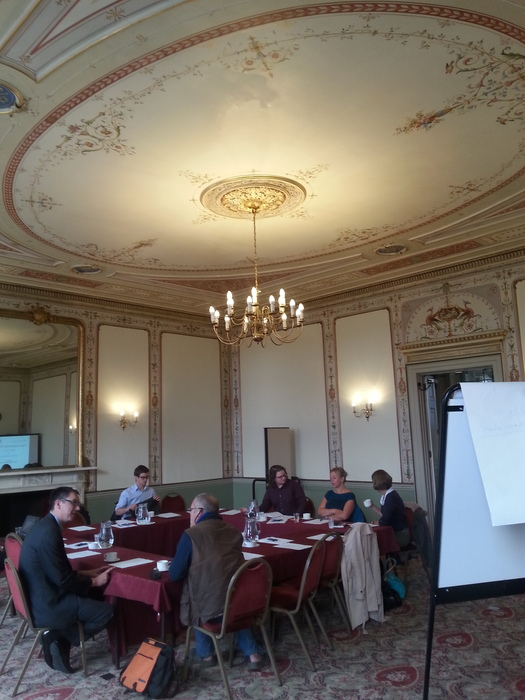
\includegraphics{img/Workshop.jpg}
 \caption{Kingston Maurward College, Dorchester}
\end{marginfigure}

The workshop was attended by ten Dorset council staff from public health and the environment directorate representing all climate change related projects in the council and two participants from the Dorset Partnership for Older People Programme.

A short presentation was made at the outset of the workshop to give the participants an update on the results of the ongoing literature review and horizon scanning work. The aim of this workshop was to garner local knowledge that can be used in the development of our Futures Story and Simulation Model outputs.

Futures Story: a narrative written for consumption by the general public about two possible futures for older people in Dorset. These stories are told from the perspective of someone living in Dorset in 2044. In the first story, the future as described is the future we are likely to get if we pursue a `business as usual approach' to how we accommodate the needs of older people and the second story focusses on our `desired future' that encapsulates what each of us want for our later years.

The workshop sessions were organised into two key topics: (1) what challenges the future holds for older people in a Dorset of 2044 (Figure~\ref{fig:op}) and (2) what public health interventions might be possible (Figure~\ref{fig:tsi}).

\begin{figure*}[htbp]
\centering
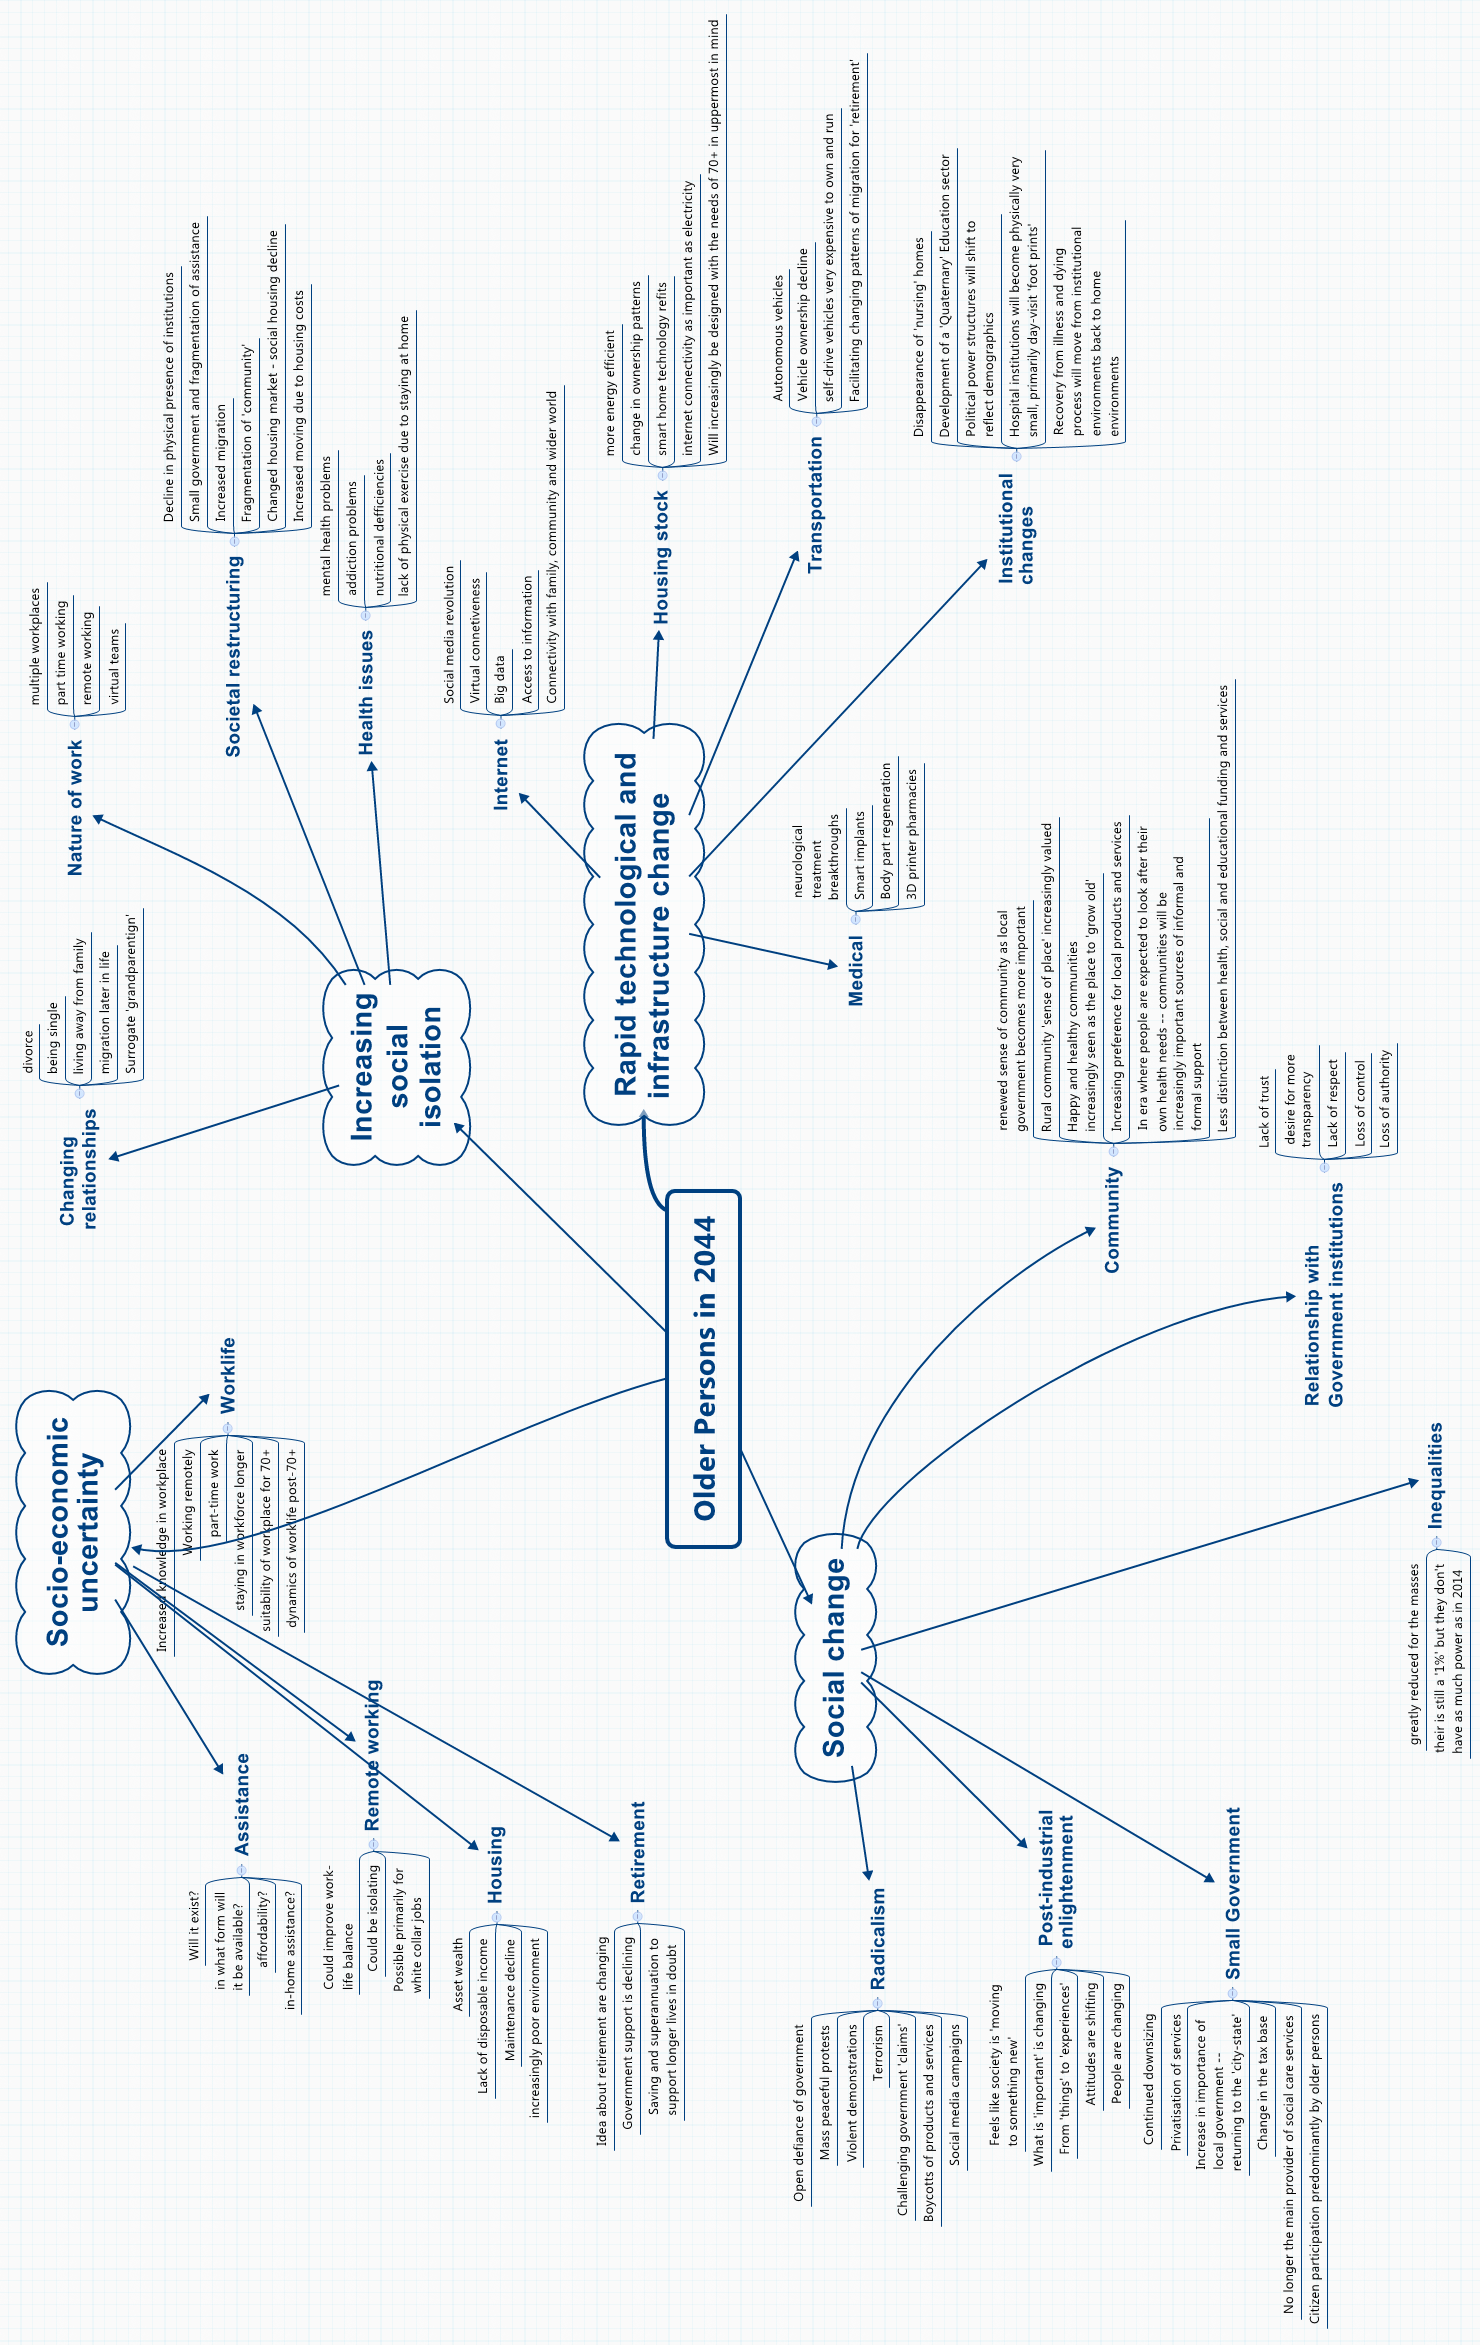
\includegraphics{img/OlderPersons2044.png}
\caption[Challenges -- Mind Map]{Challenges to be faced by older people in a Dorset of 2044 (mind map is also available in Xmind format).\label{fig:op}}
\end{figure*}

\begin{figure*}[htbp]
\centering
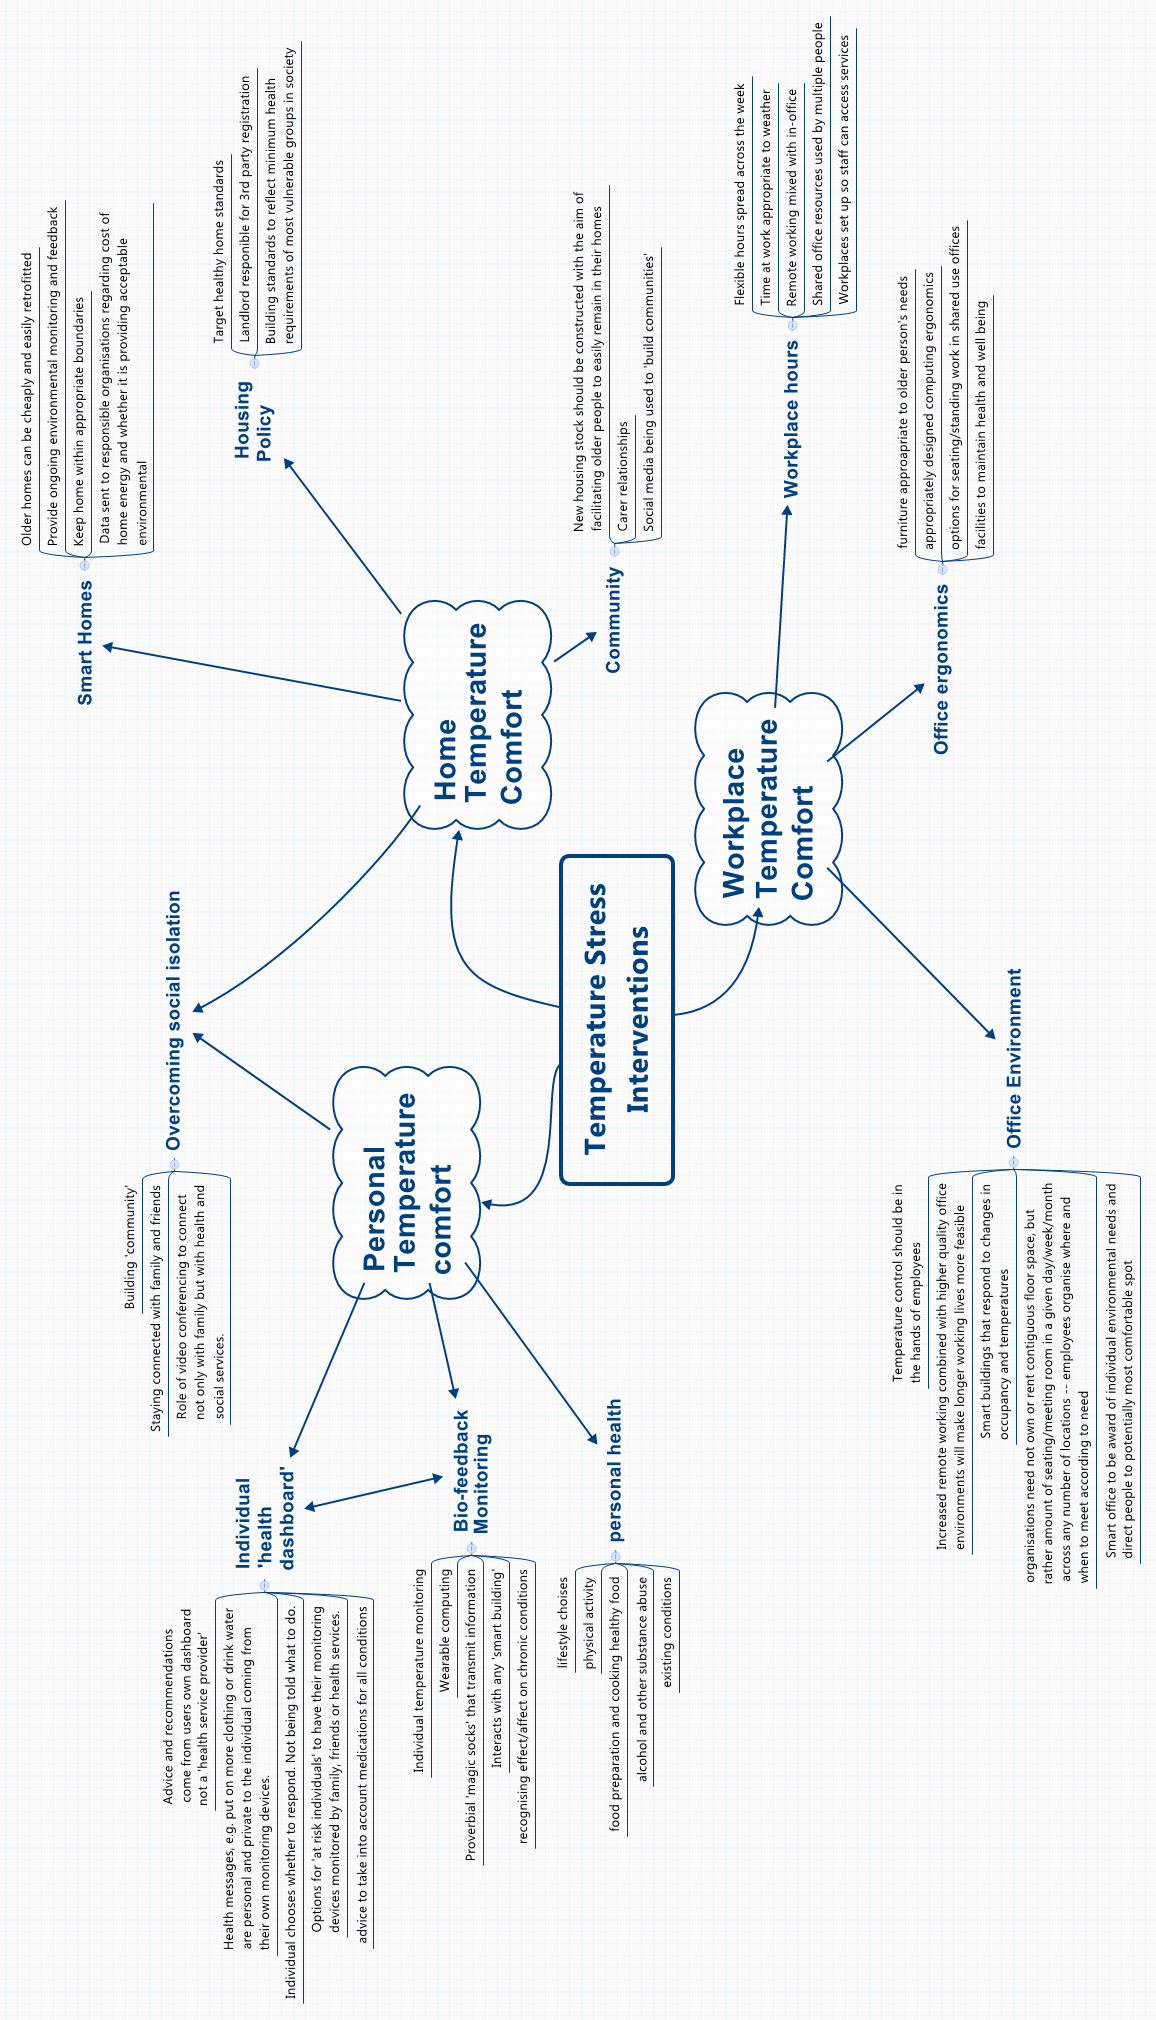
\includegraphics{img/TemperatureStressInterventions.png}
\caption[Public Health Interventions -- Mind Map]{Public health interventions aimed at mitigating the impacts of climate change on older people in Dorset, 2044  (mind map is also available in Xmind format).\label{fig:tsi}}
\end{figure*}

Simulation Model: a systems thinking tool that participants and stakeholders will be able to interact with in order to get a better idea of how the key public health levers can be manipulated to mitigate the impact of climate change on older people in Dorset. Our working model was subsequently improved and a new version will be prepared early next year for eventual use in stakeholder engagement and will be detailed in the final report (Figure~\ref{fig:smv2}).

\begin{figure*}[htbp]
\centering
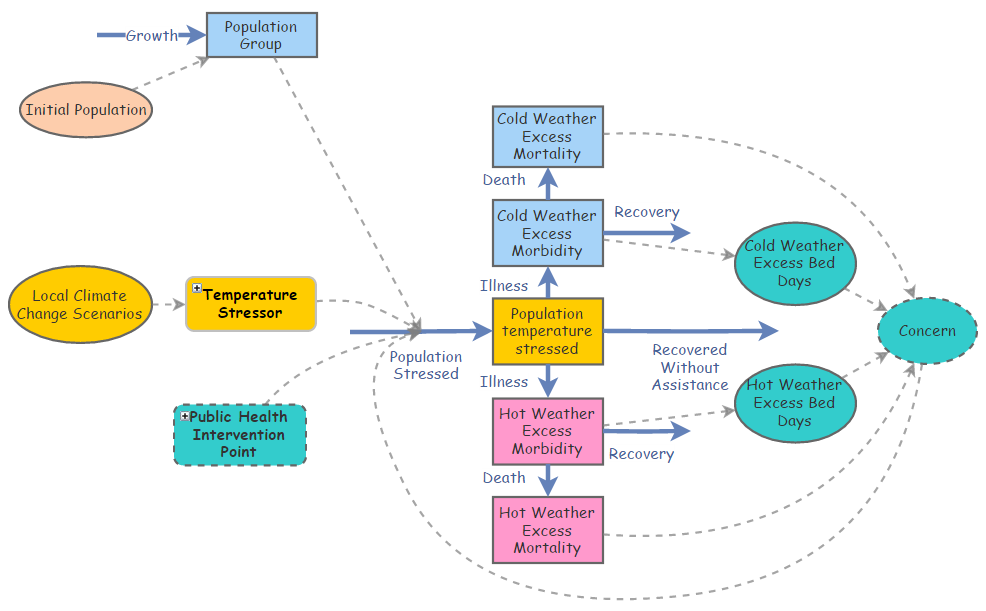
\includegraphics{img/InterventionSystemModelv2.png}
\caption[Insight Maker Model]{A systems model representing potential impacts of climate change on older people in Dorset of 2044 (The model can be accessed here: https://insightmaker.com/insight/17406).}
\label{fig:smv2}
\end{figure*}

\section{Workshop Outcomes}
The participants contributed valuable insight that was captured during our cognitive mapping exercises relating to the expected challenges older people in Dorset will face in 2044 and potential interventions. The challenge to the workshop group as a whole was shifting our thinking from what is happening today in Dorset to that which may be happening 30 years hence. It required a degree of `out of the box thinking' on the part of participants and an ability to continually refresh a `contextual society' that will change considerably from that recognised today. The participants were primed at the outset of the workshop with identified trends in working life-retirement, health technology, wider society, and government function including macroeconomics. The writing of the futures story and continuation of the simulation model development that were aided by this workshop will be completed in February 2015.

\section{Workshop Organisation}

Exploring the Future of Older People in Dorset:\\ 
Responding to Climate Change\\
23rd October, 2014: 9.30am--1.30pm\\
Kingston Maurward College, Dorchester\\

How often do we seriously contemplate the future?  The planning of services and development of policy usually focuses on improving outcomes within a relatively short time period, perhaps a year or two.  Sometimes however an issue forces us to think longer-term, over decades, and climate change is one of these.  For West Dorset we need to consider hotter, drier summers; warmer, wetter winters along with increased likelihood of storms and flooding, heat waves and droughts.  The impact of these changes are unlikely to be felt equally across communities, and there is a particular concern about how well older people will be able to adapt and thrive in these circumstances. 

Through a dynamic process of participation, this workshop aims to build scenarios, describing the Dorset of 2044 with a focus on the lives of older people (aged 70+), and most importantly identifying a preferred future in the face of climate change.  We are inviting stakeholders from a broad range of backgrounds with insight into the needs of older people and the challenges we face with extreme weather events.

Participants (as well as others with an interest) are asked to complete an online survey prior to attending the workshop, the results of which we will consider on the day.  The survey is entirely anonymous and, depending on the level of detail, will take 30-45 minutes to complete. Click \url{https://www.surveymonkey.com/s/G3HNMYG}{https://www.surveymonkey.com/s/G3HNMYG} to access the online survey.

Please complete by 25th September. Please confirm your attendance or otherwise with Joanna Joy at j.joy@dorsetcc.gov.uk by 25th September

LUNCH and REFRESHMENTS will be provided on the day!

The event is being organised by Public Health Dorset as part of a local climate adaptation project.  It is supported by the Big Lottery Fund and is a component of the wider programme `Communities Living Sustainably' in Dorset. 

\section{Workshop Notes}

Apologies: Rob Darrington, Jackie Allen, Derek Lake, George Gibson

Present: Rachel Partridge, Chris Ricketts, Rebecca Pearce, Emma Wilson, Dave Lemon, Public Health Dorset, DCC; Rupert Lloyd - Sustainability Team, DCC; Jon Bird - Energy Efficiency Development Officer, Environment Directorate, DCC; Sue Warr - Strategic Commissioning Manager, Programme Manager - Dorset POPP, DCC; Dominic Knorpel - POPP (Rylands Farm with older people); Chris Skelly, SkelINTEL Consulting

\subsection{Breakout Session 1: Mapping our futures -- Priority trends}
These bullet points summarise the priority trends identified by during the first breakout session (Figures~\ref{fig:mindmap1}--\ref{fig:mindmap4}).

\begin{enumerate}
\item Physical infrastructure
\begin{itemize}
\item Buildings and roads -- suitable for people of old ages
\item Transport links -- rethink nationally
\end{itemize}
\item Socio economic
\begin{itemize}
\item Working together
\item Training for retirement
\item Work/life balance
\item Active and engaged with society
\item People wanting to be cognitively active in old age years -- uni of 3rd age
\item Physical relationships
\item Industrial revolution
\end{itemize}
\item Population health 
\begin{itemize}
\item Rurality issue -- difficult to get access to services
\item People's own responsibility for health and wellbeing
\end{itemize}
\end{enumerate}

\begin{figure*}[htpb]
 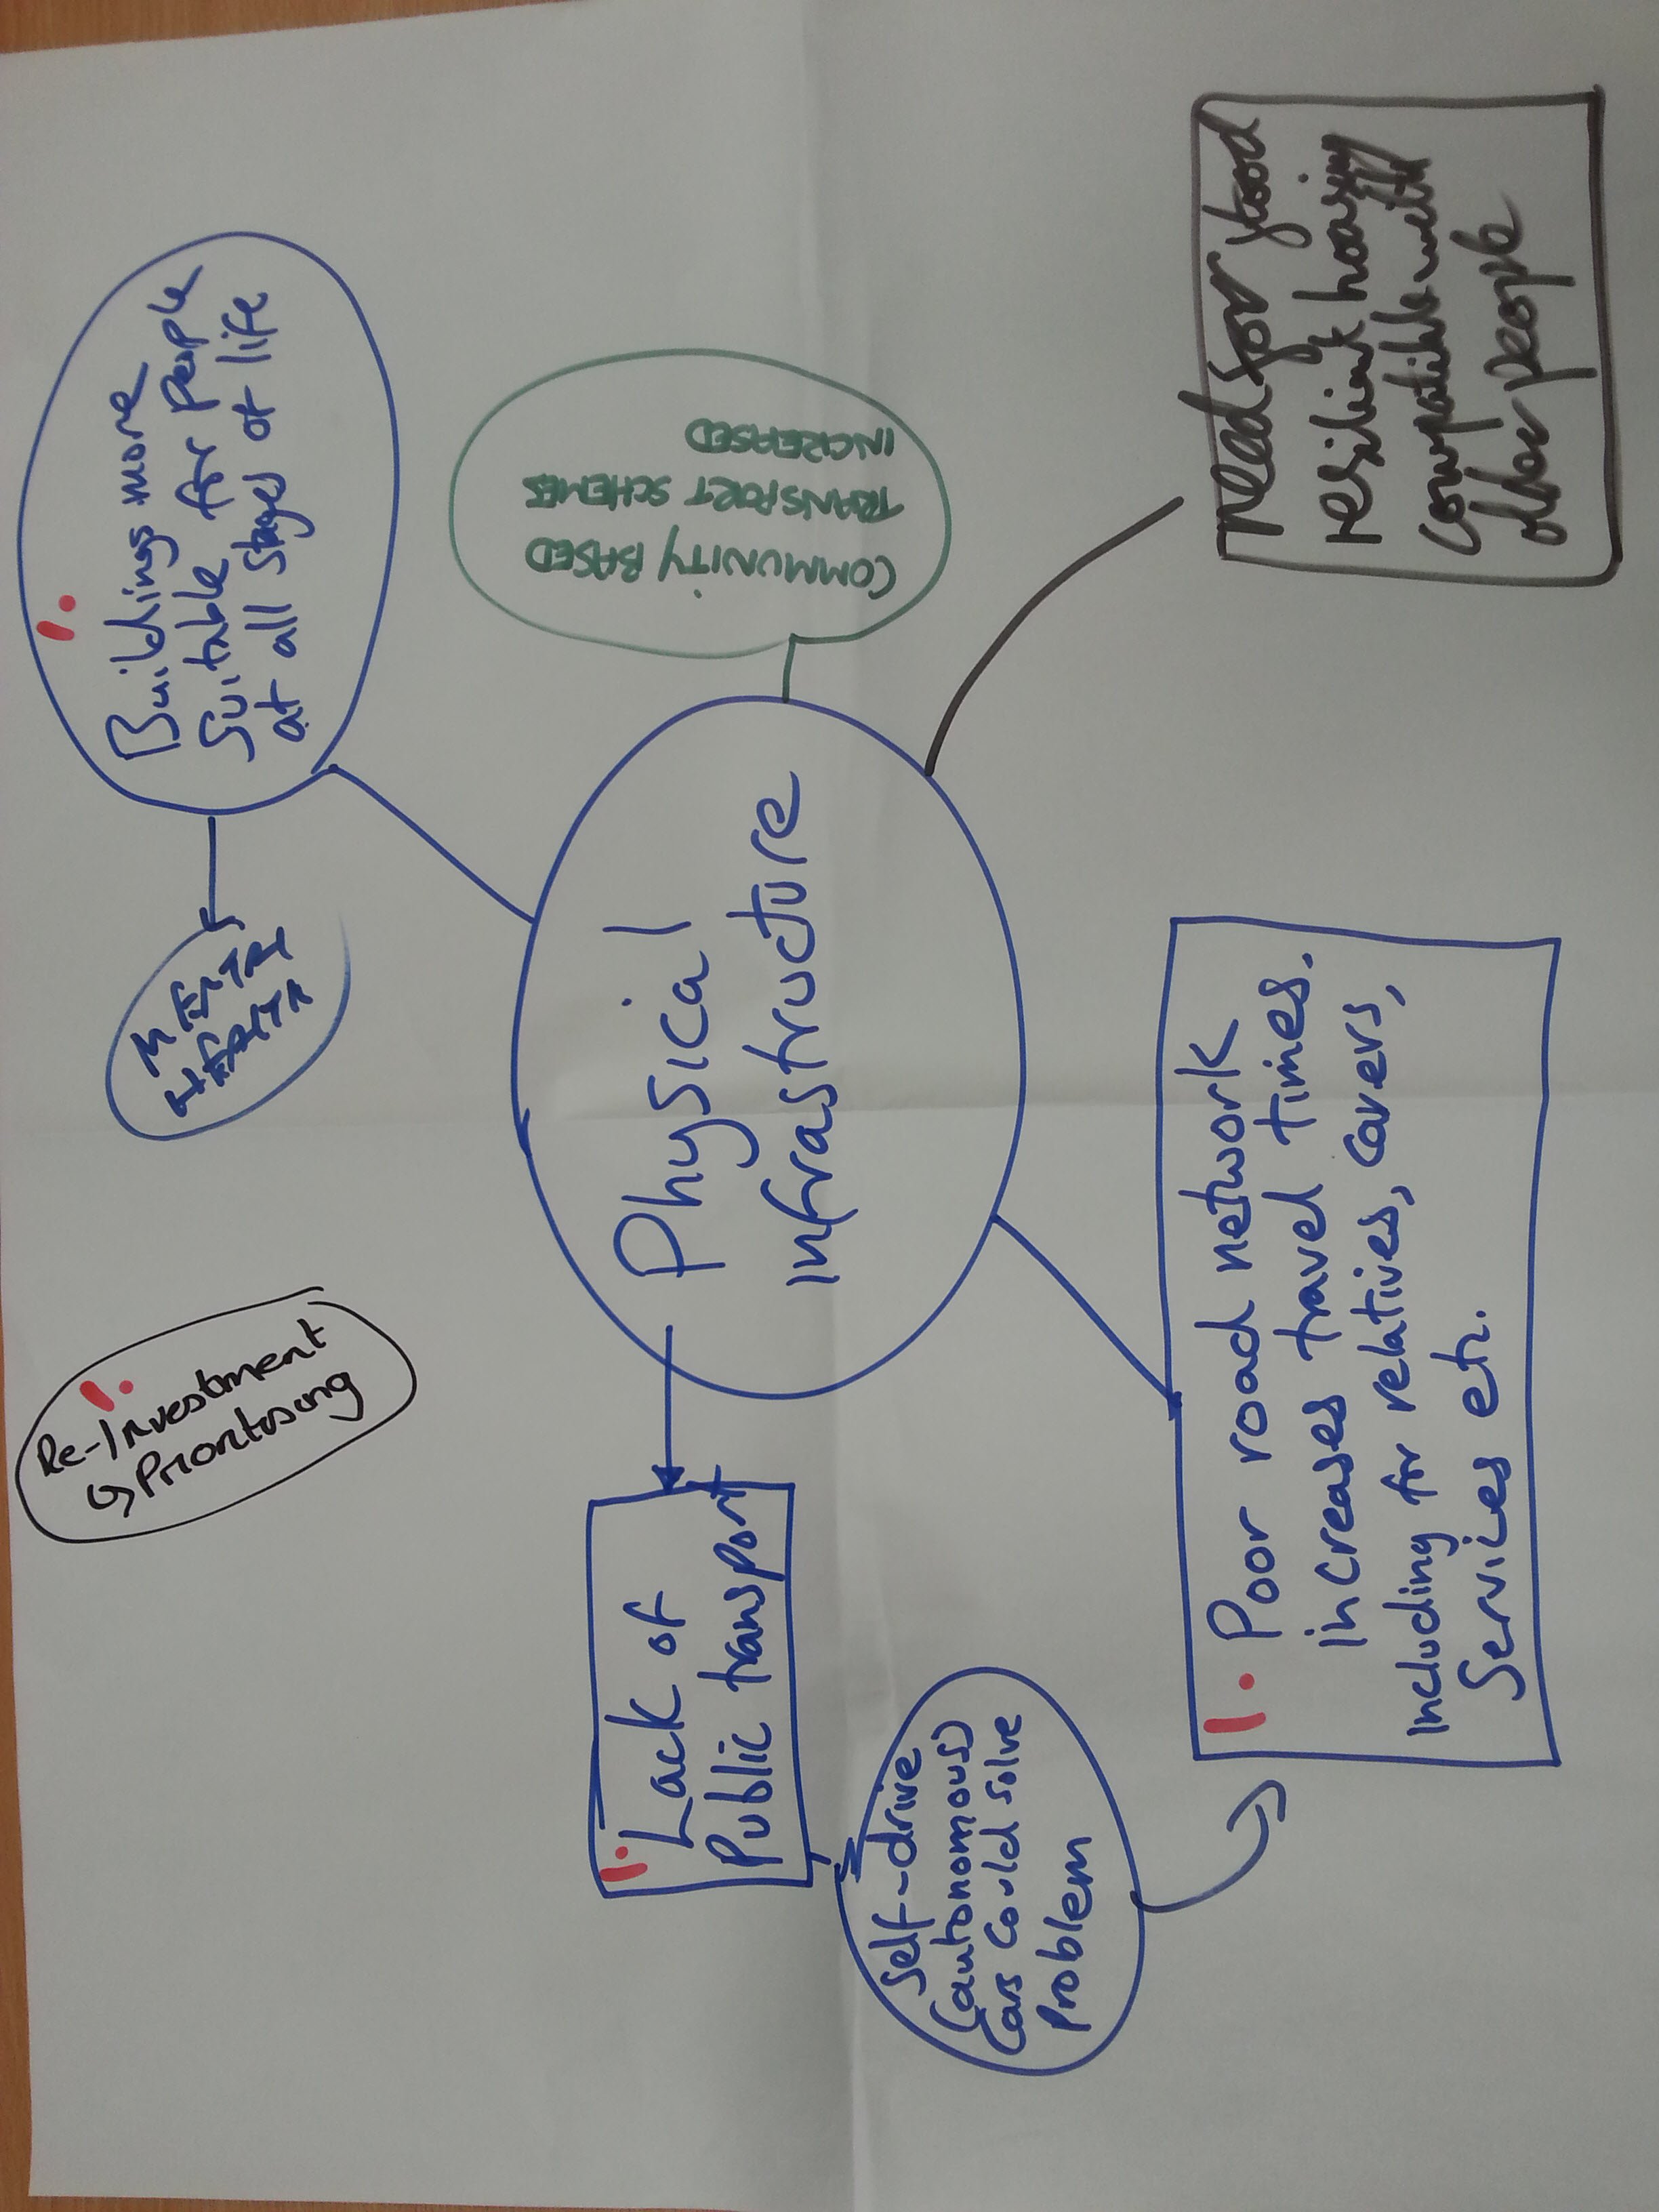
\includegraphics{img/wb1.jpg}
 \caption[Priority Trends: Group 1]{Priority Trends: mind mapping by breakout Group 1.\label{fig:mindmap1}}
\end{figure*}

\begin{figure*}[htpb]
 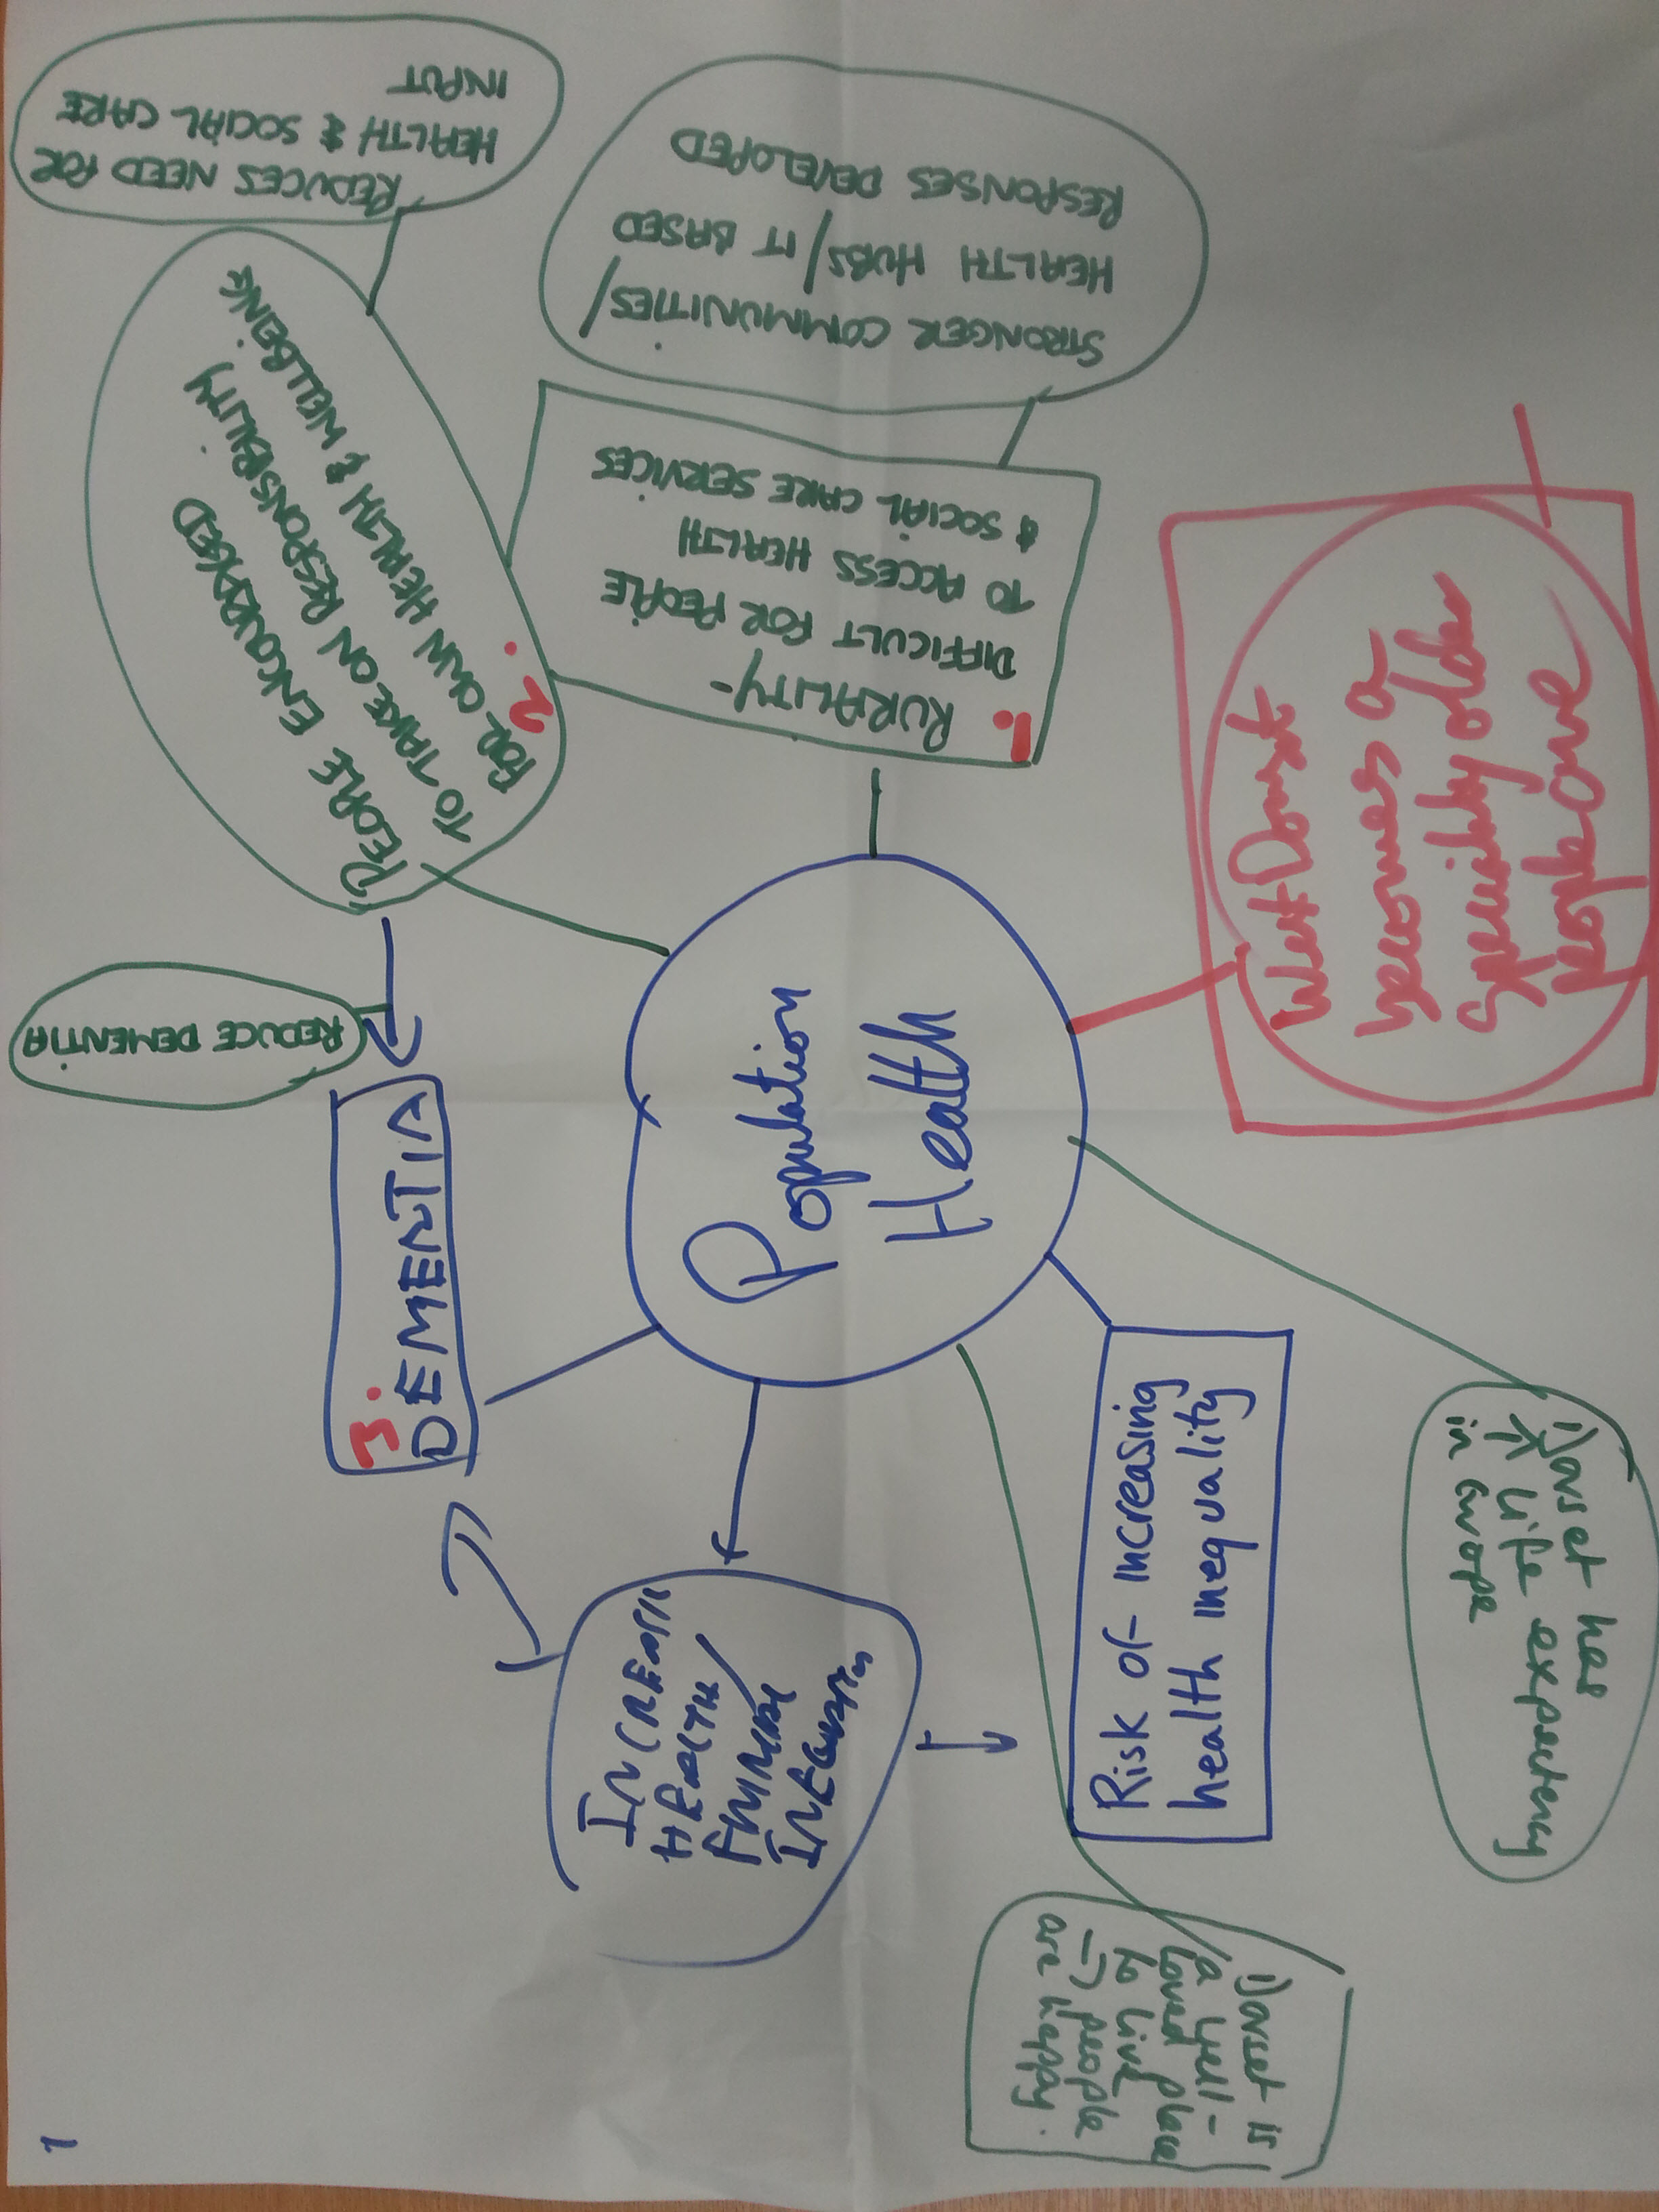
\includegraphics{img/wb2.jpg}
  \caption[Priority Trends: Group 2]{Priority Trends: mind mapping by breakout Group 2.\label{fig:mindmap2}}
\end{figure*}

\begin{figure*}[htpb]
 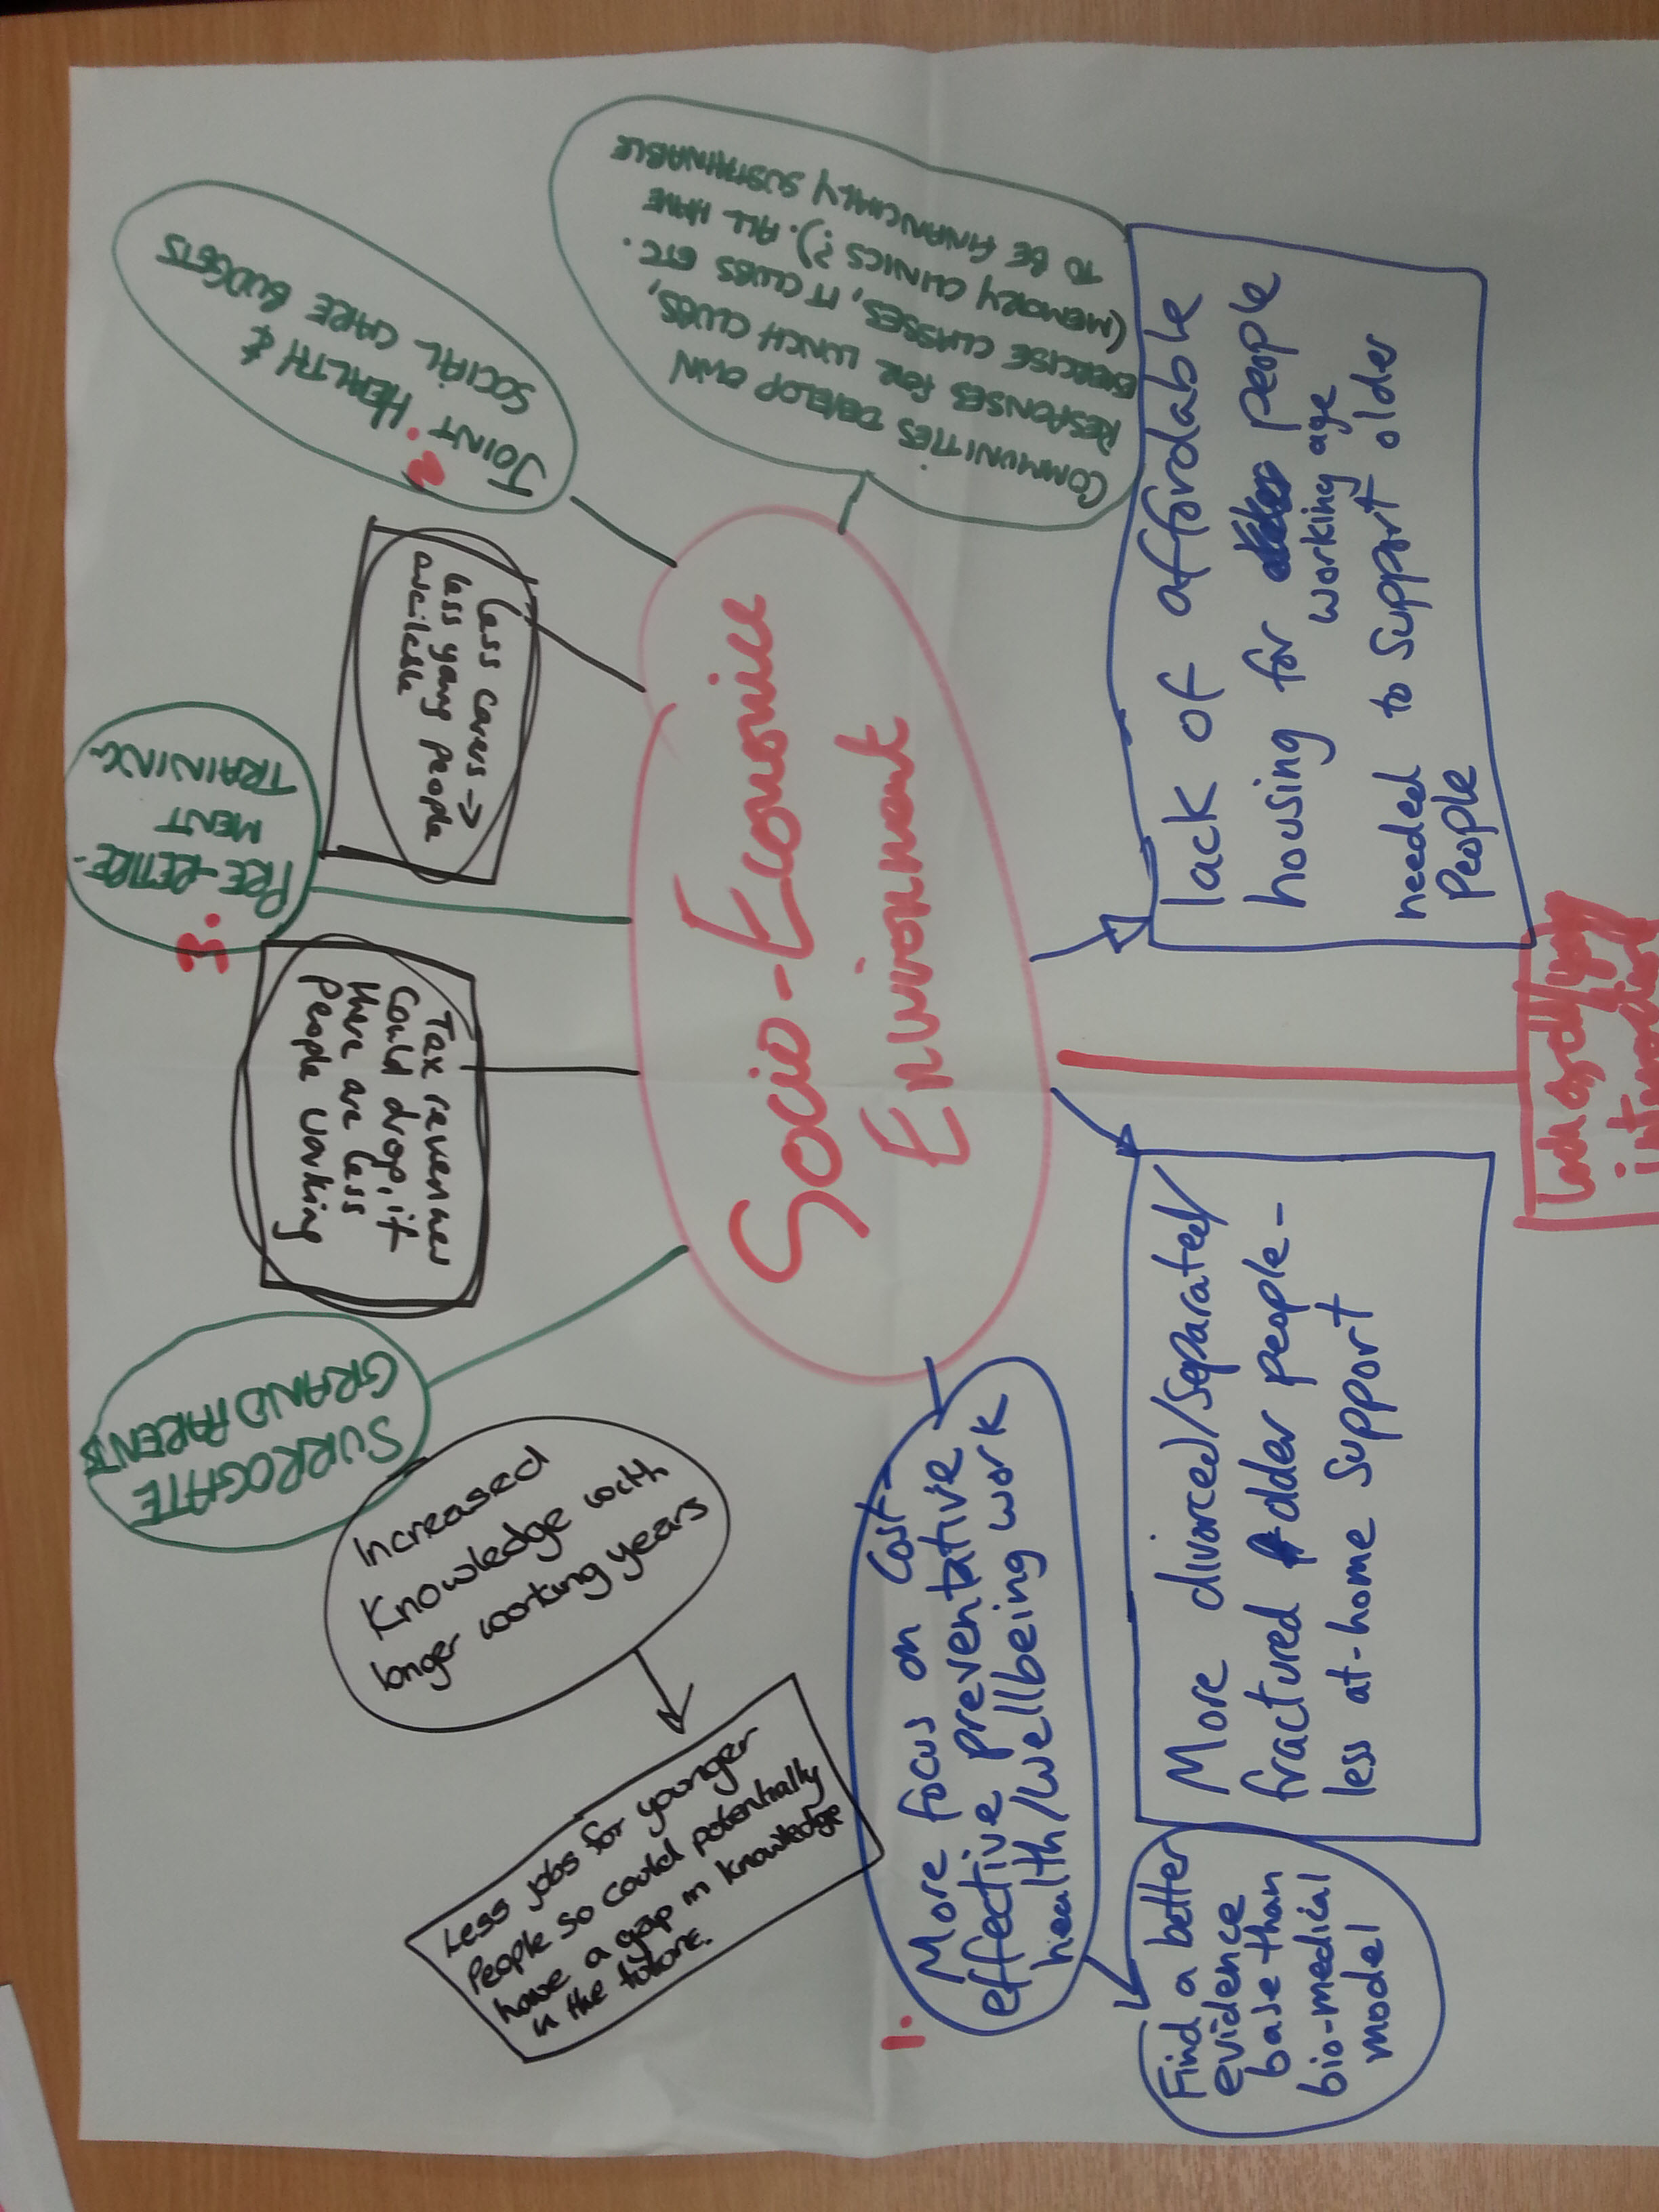
\includegraphics{img/wb3.jpg}
  \caption[Priority Trends: Group 3]{Priority Trends: mind mapping by breakout Group 3.\label{fig:mindmap3}}
\end{figure*}

\begin{figure*}[htpb]
 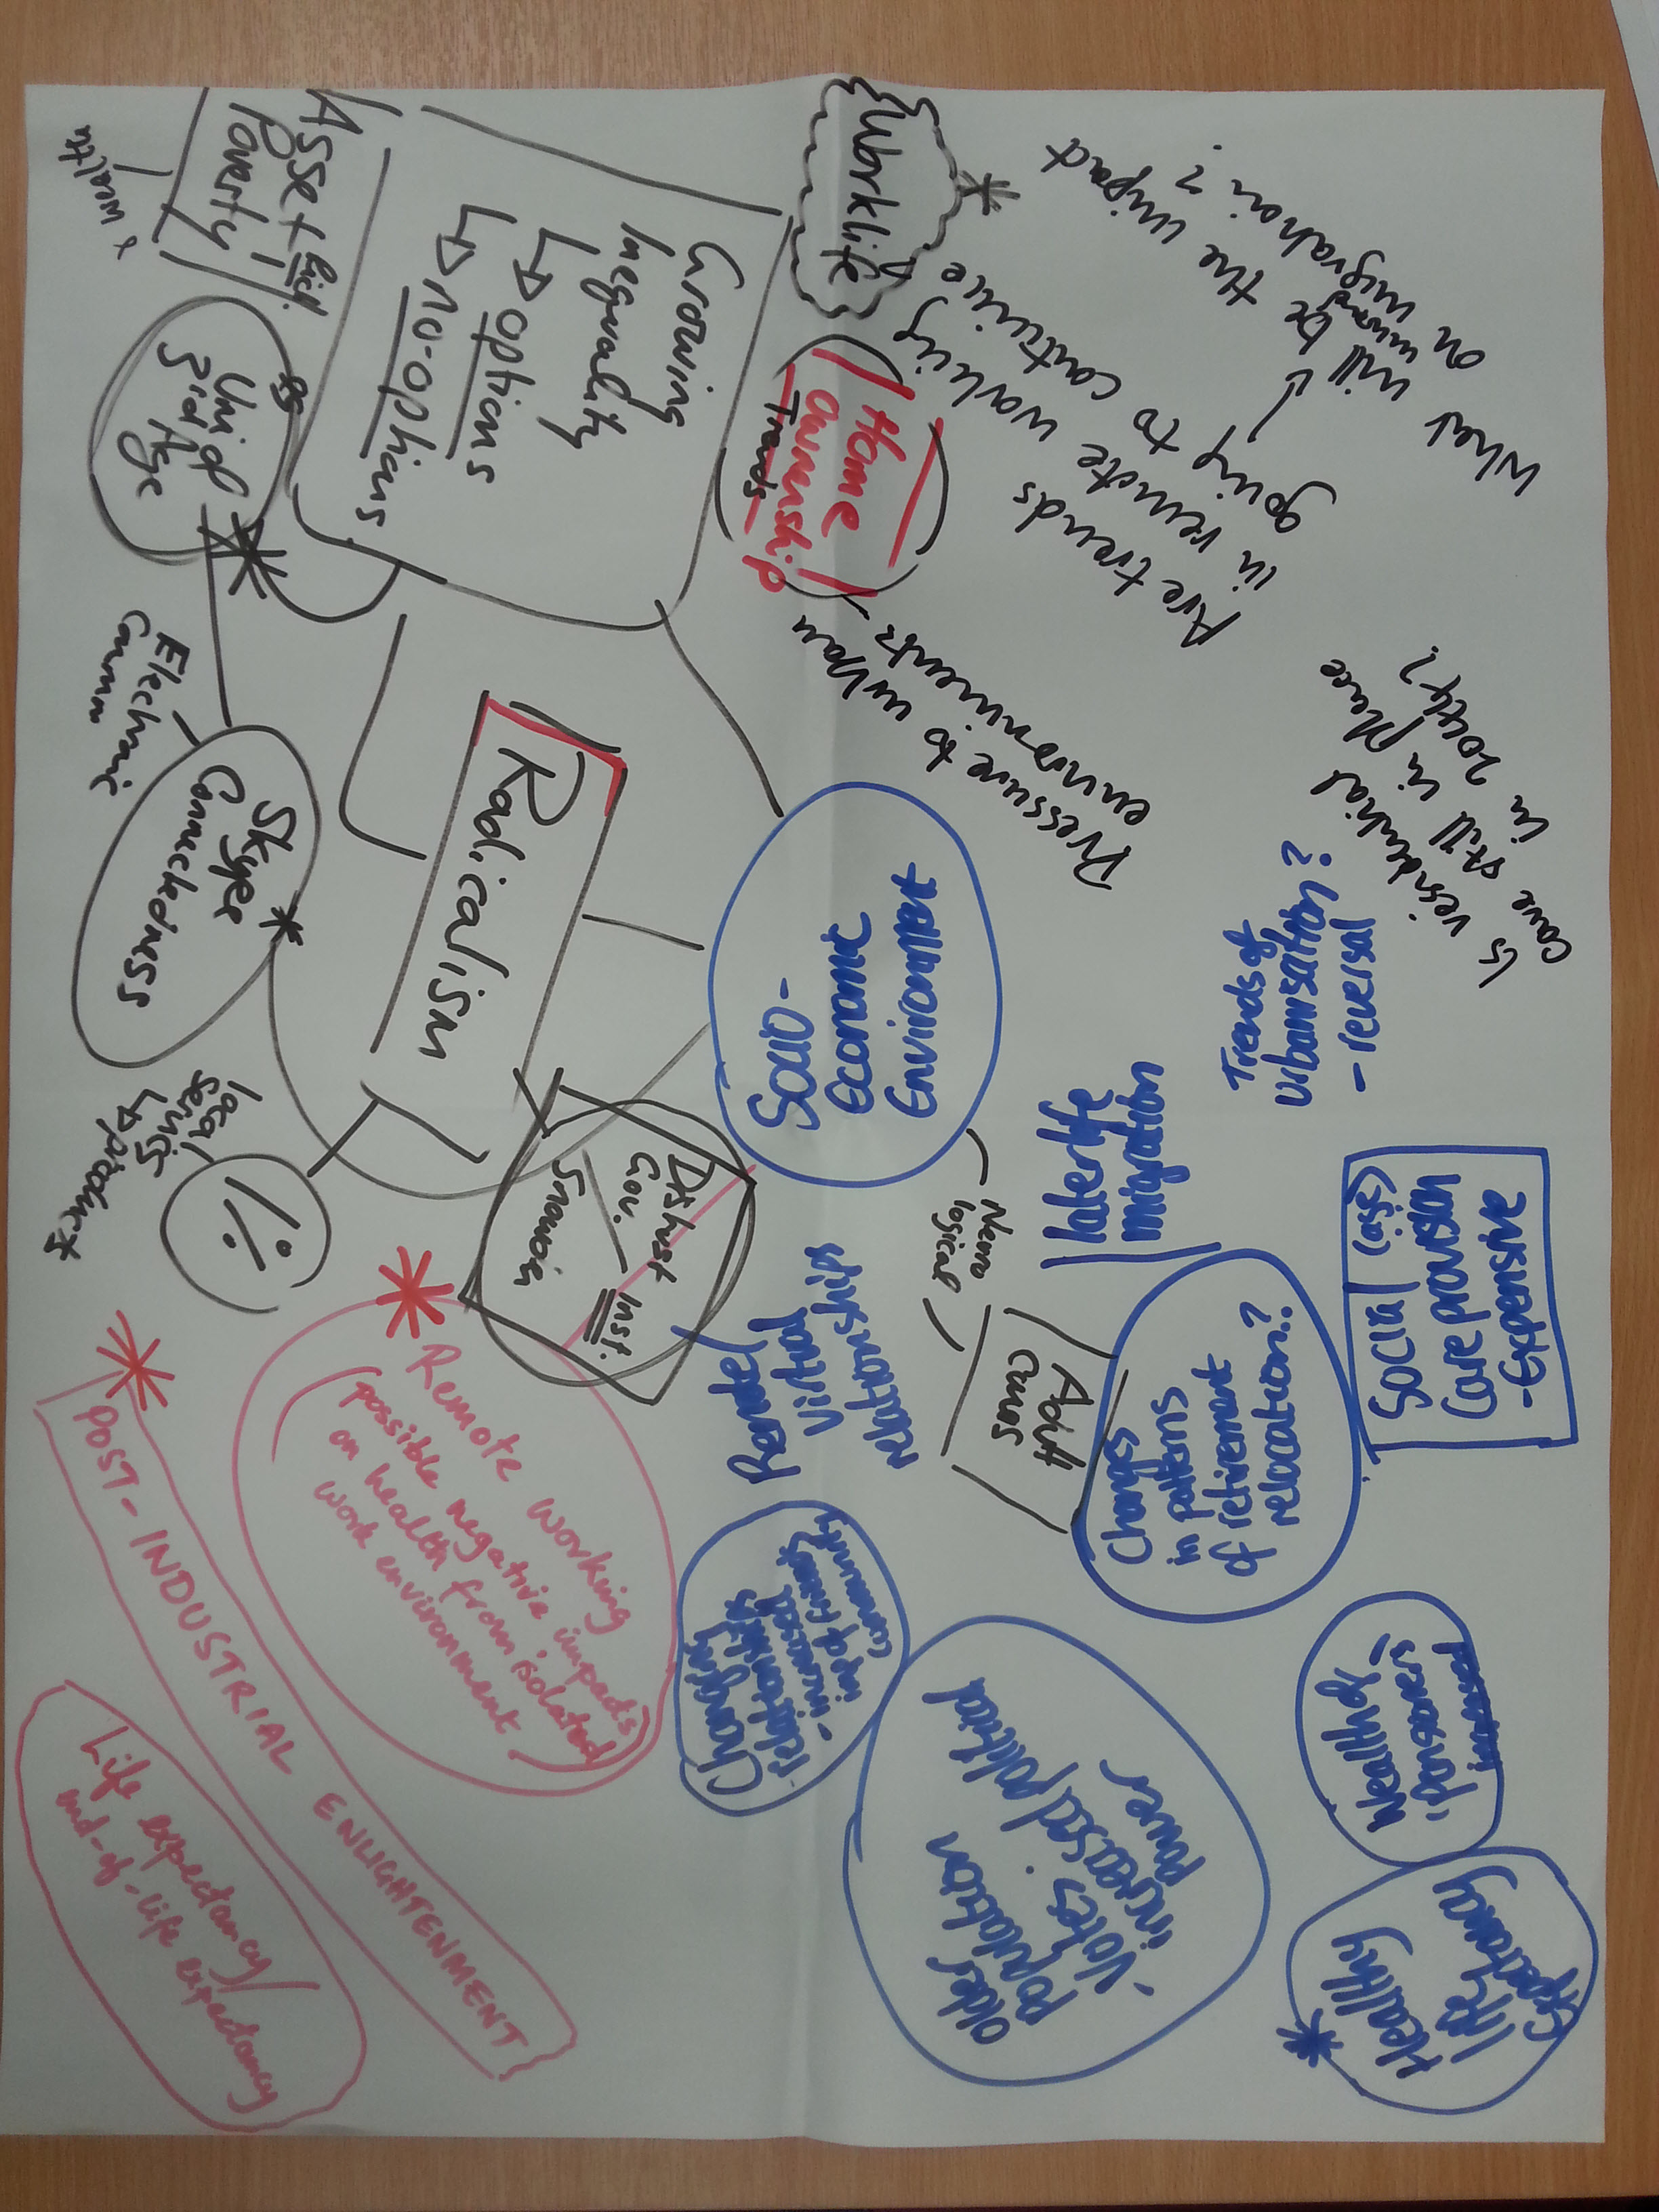
\includegraphics{img/wb4.jpg}
  \caption[Priority Trends: Group 4]{Priority Trends: mind mapping by breakout Group 4.\label{fig:mindmap4}}
\end{figure*}


\subsection{Breakout Session 2: Identifying Public Health Interventions}
These bullet points summarise the potential public health interventions identified by during the second breakout session (Figures~\ref{fig:mindmap5}--\ref{fig:mindmap8}).

\begin{enumerate}
\item Pre discussions:
\begin{itemize}
\item Body mass -- does weight on mean warmer beings?
\item Socialisation-- heat wave abandonment 
\item Population getting used to more IT based activities
\end{itemize}
\item Rebecca's Group -- Reducing number exposed: Intervention A
\begin{itemize}
\item Exposure in home / exposure outside of home
\item Home MOTs, devices that could let you know if it's too cold, general home improvements, SAIL (Safe and Independent Living) form -- offers residents free support, services or information to help keep them safe and independent in their own home.
\item Planting trees -- benches underneath for shade
\item Alerts for upcoming cold spells
\item Nutrition -- advice and supply
Number recovered: Intervention B
\item Reduce length of stay in hospital -- re-housing, SAIL form, pubs, pharmacies, community centres -- more social environment -- food, warmth, social aspect
\end{itemize}
\item Rachel's Group -- Number recovered:
\begin{itemize}
\item Magic socks (rings, bracelet) -- monitoring body temperature -- technology to feed back to individual or third party about temperatures and when to take action
\item Monitors within home -- hub within home detailing body temperatures, energy within home
\item Making people realise that it is an important issue -- reminders about wearing longjohns etc.
\item Clothing technology
\item Changing people's perception -- doing things for yourself
\end{itemize}
\item Numbers exposed:
\begin{itemize}
\item Awareness that it's a serious health concern
\item Getting an idea of how many people are exposed -- nature of exposure (type of medication, disease)
\item Evidence base around warming people up and cooling people down
\item Voice of authority -- older generation would have listened to someone in uniform, whereas younger generation listens to what the computer/smartphone says
\end{itemize}
\end{enumerate}

\begin{figure*}[htpb]
 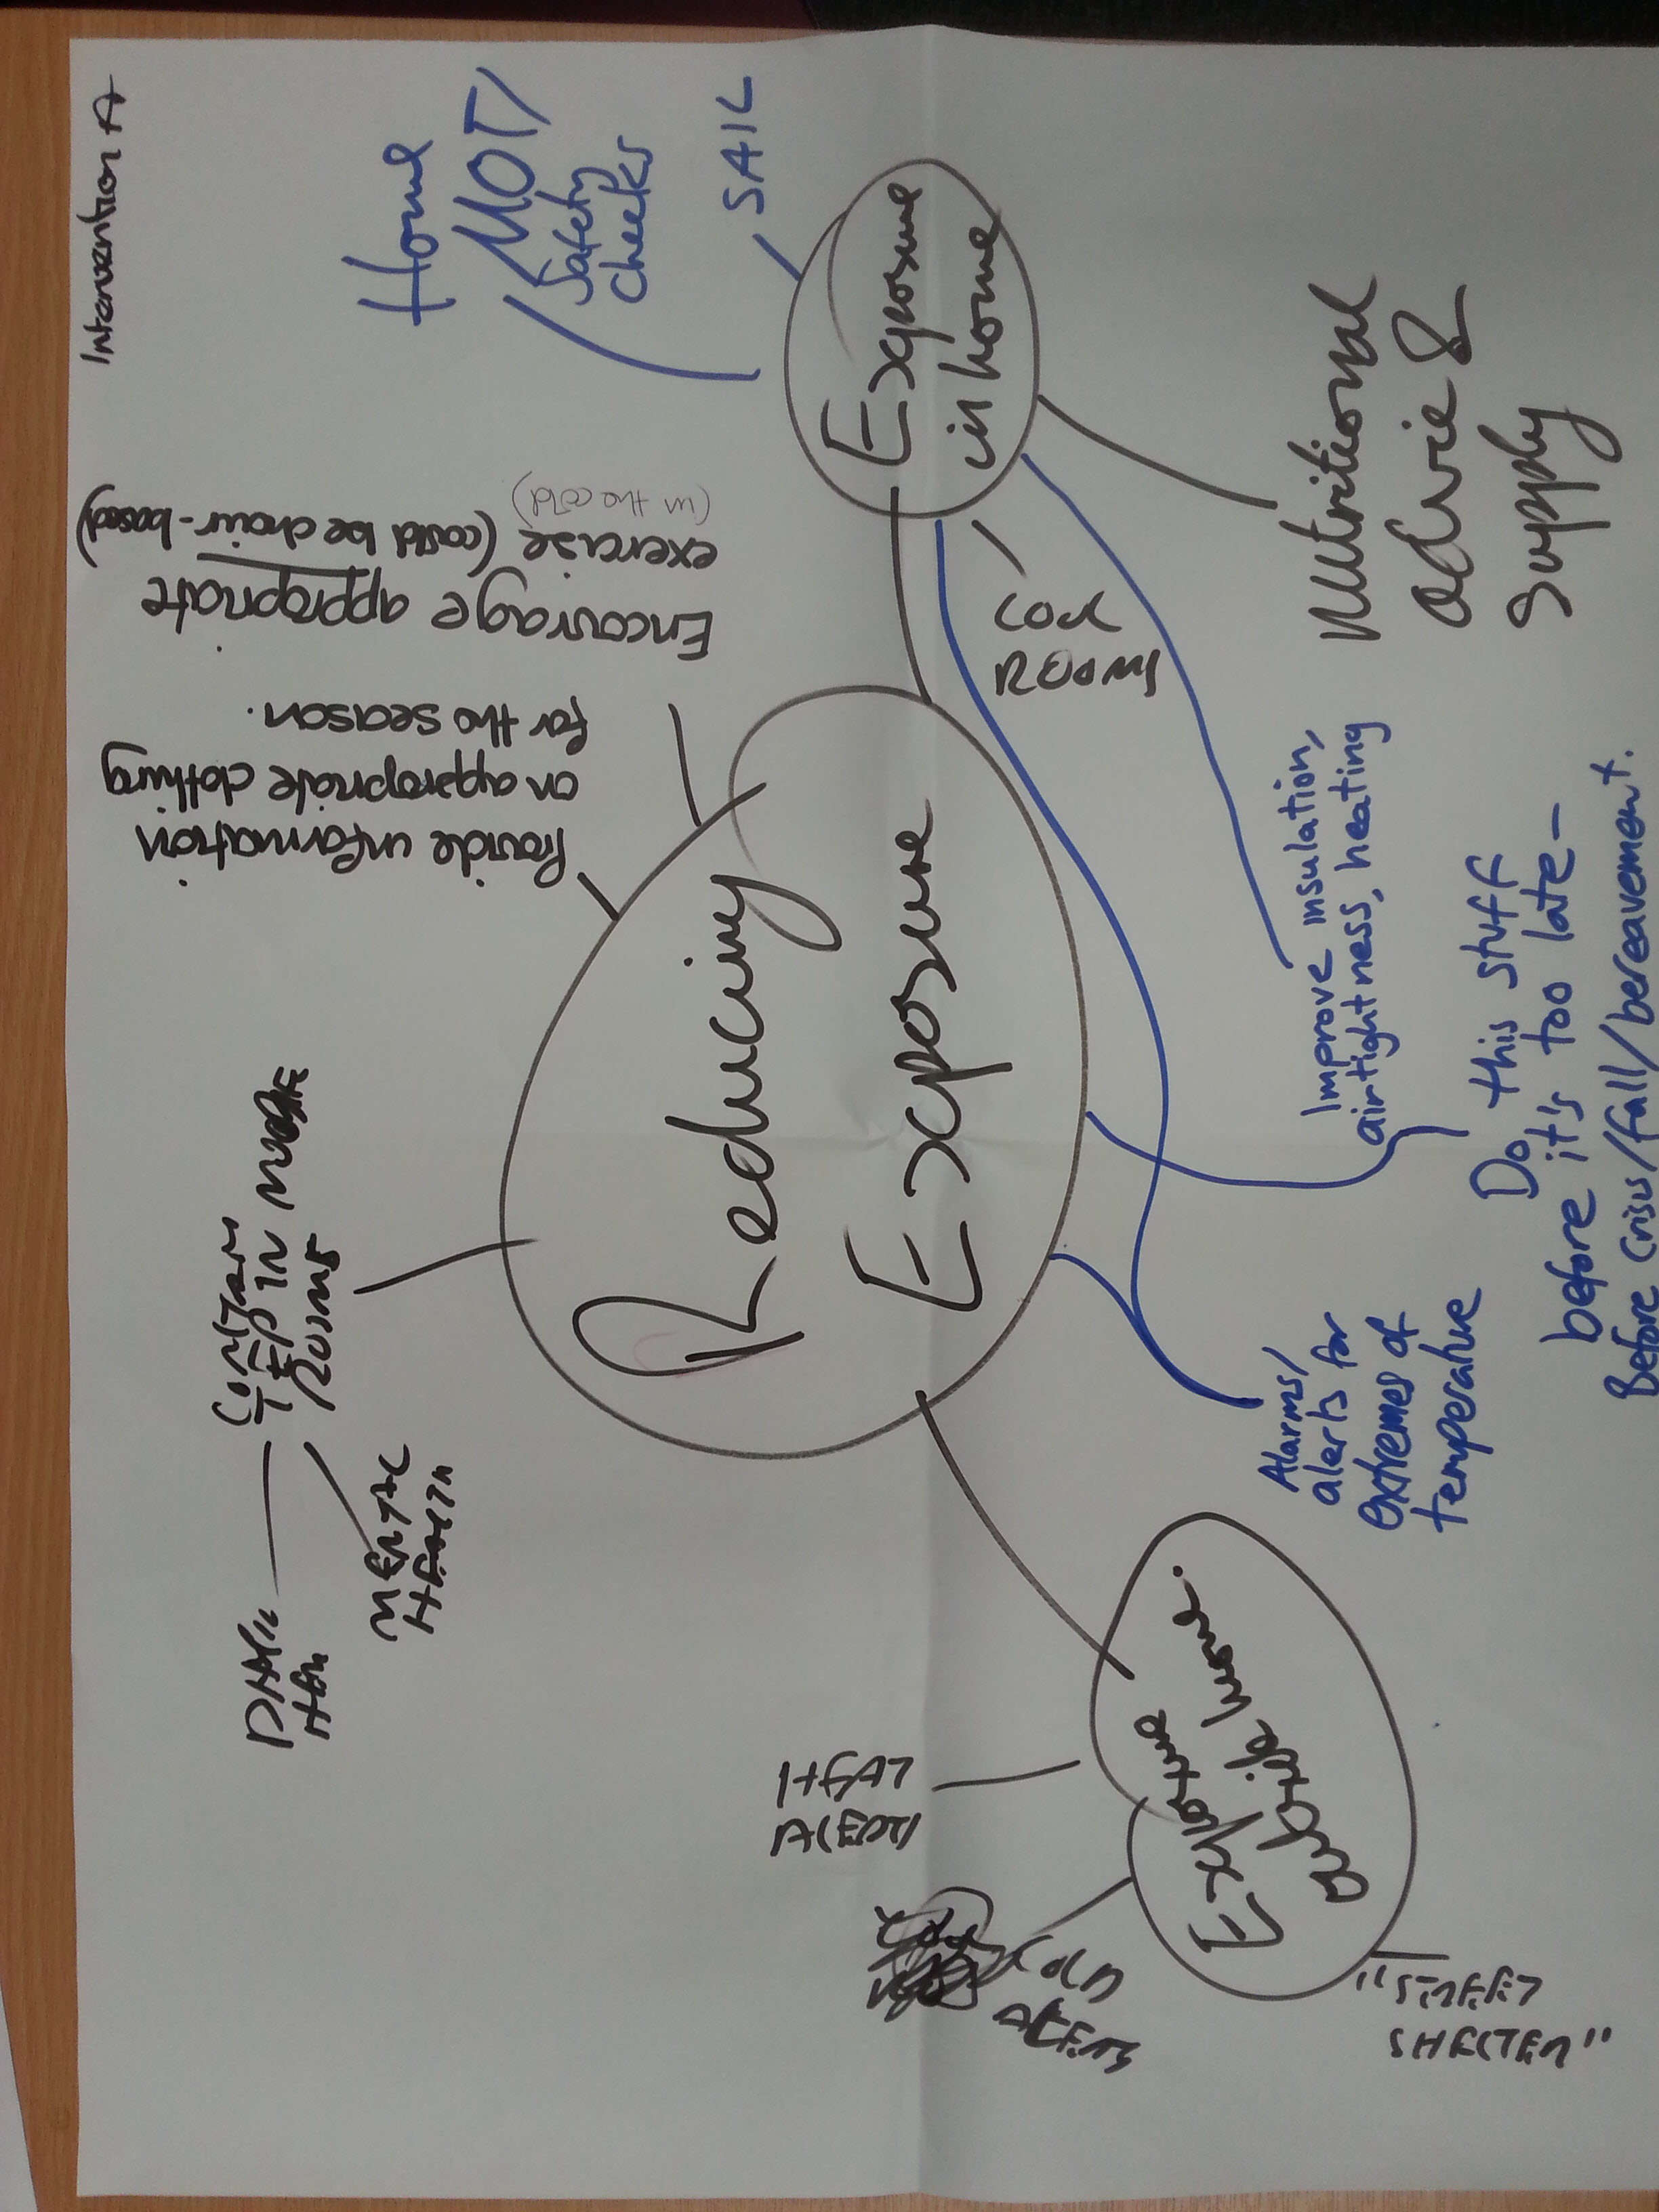
\includegraphics{img/wb5.jpg}
 \caption[Public Health Interventions: 1]{Public Health Interventions: Group 1.\label{fig:mindmap5}}
\end{figure*}

\begin{figure*}[htpb]
 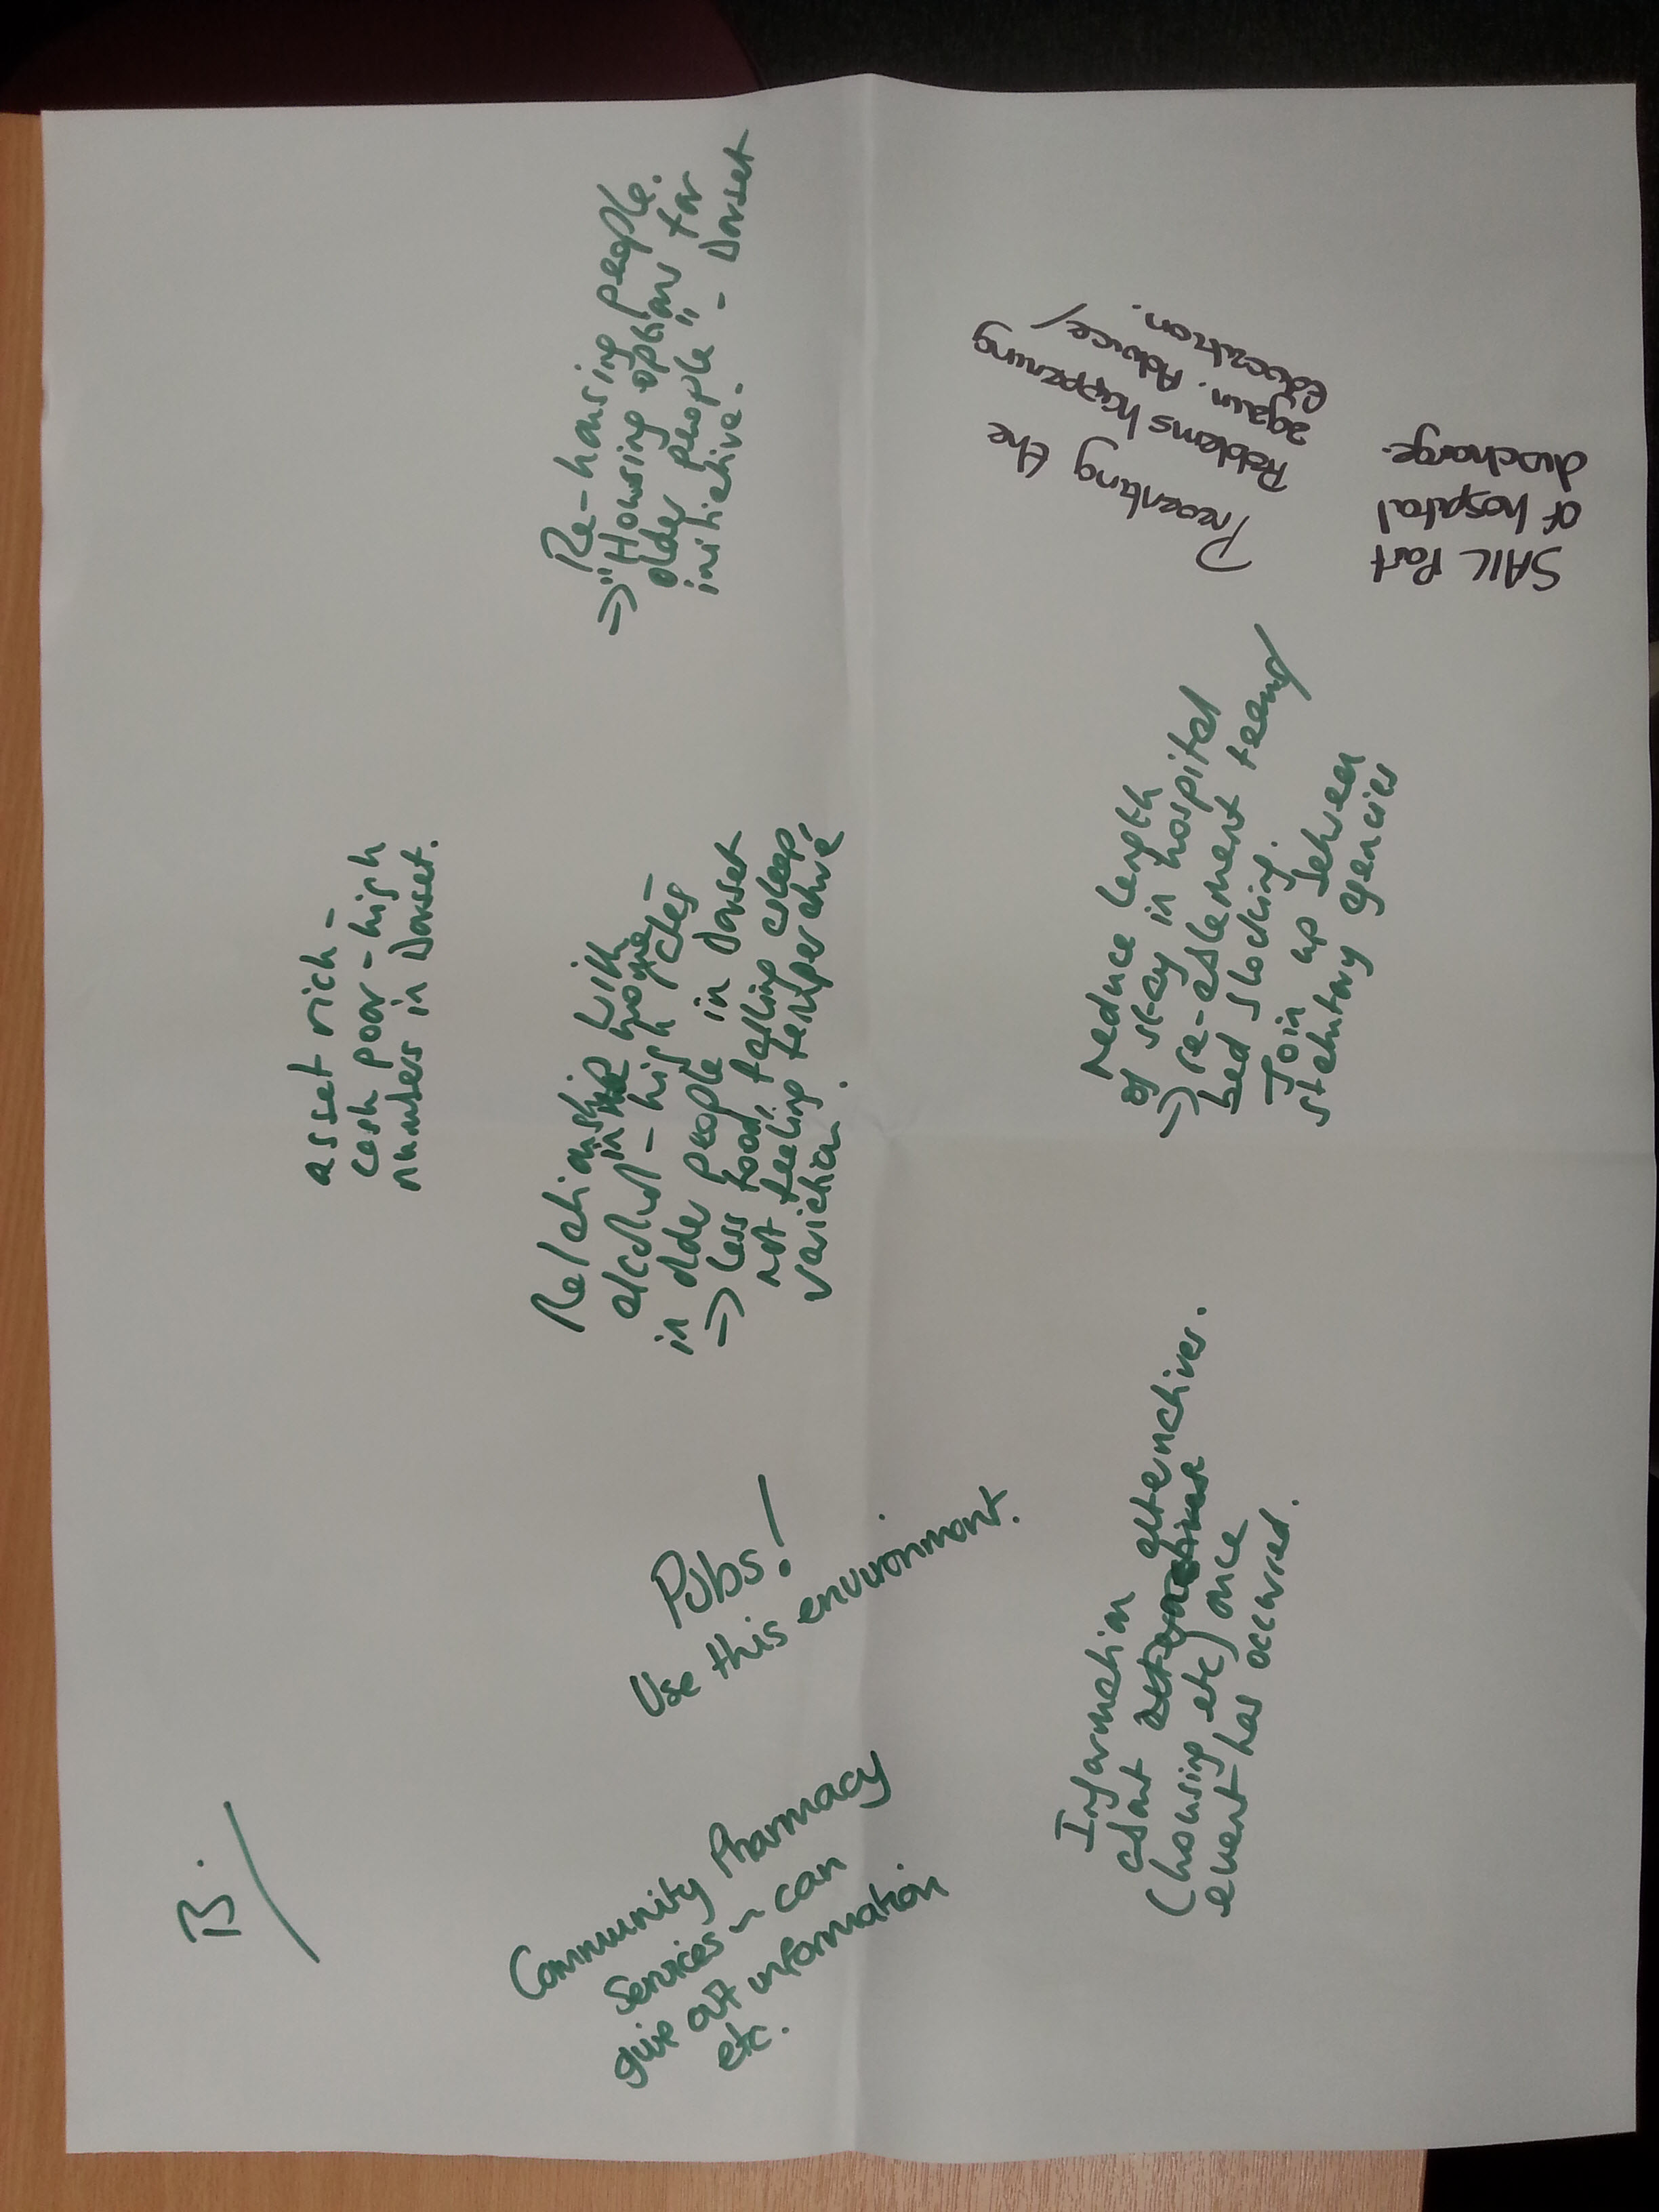
\includegraphics{img/wb6.jpg}
  \caption[Public Health Interventions: 2]{Public Health Interventions: Group 2.\label{fig:mindmap6}}
\end{figure*}

\begin{figure*}[htpb]
 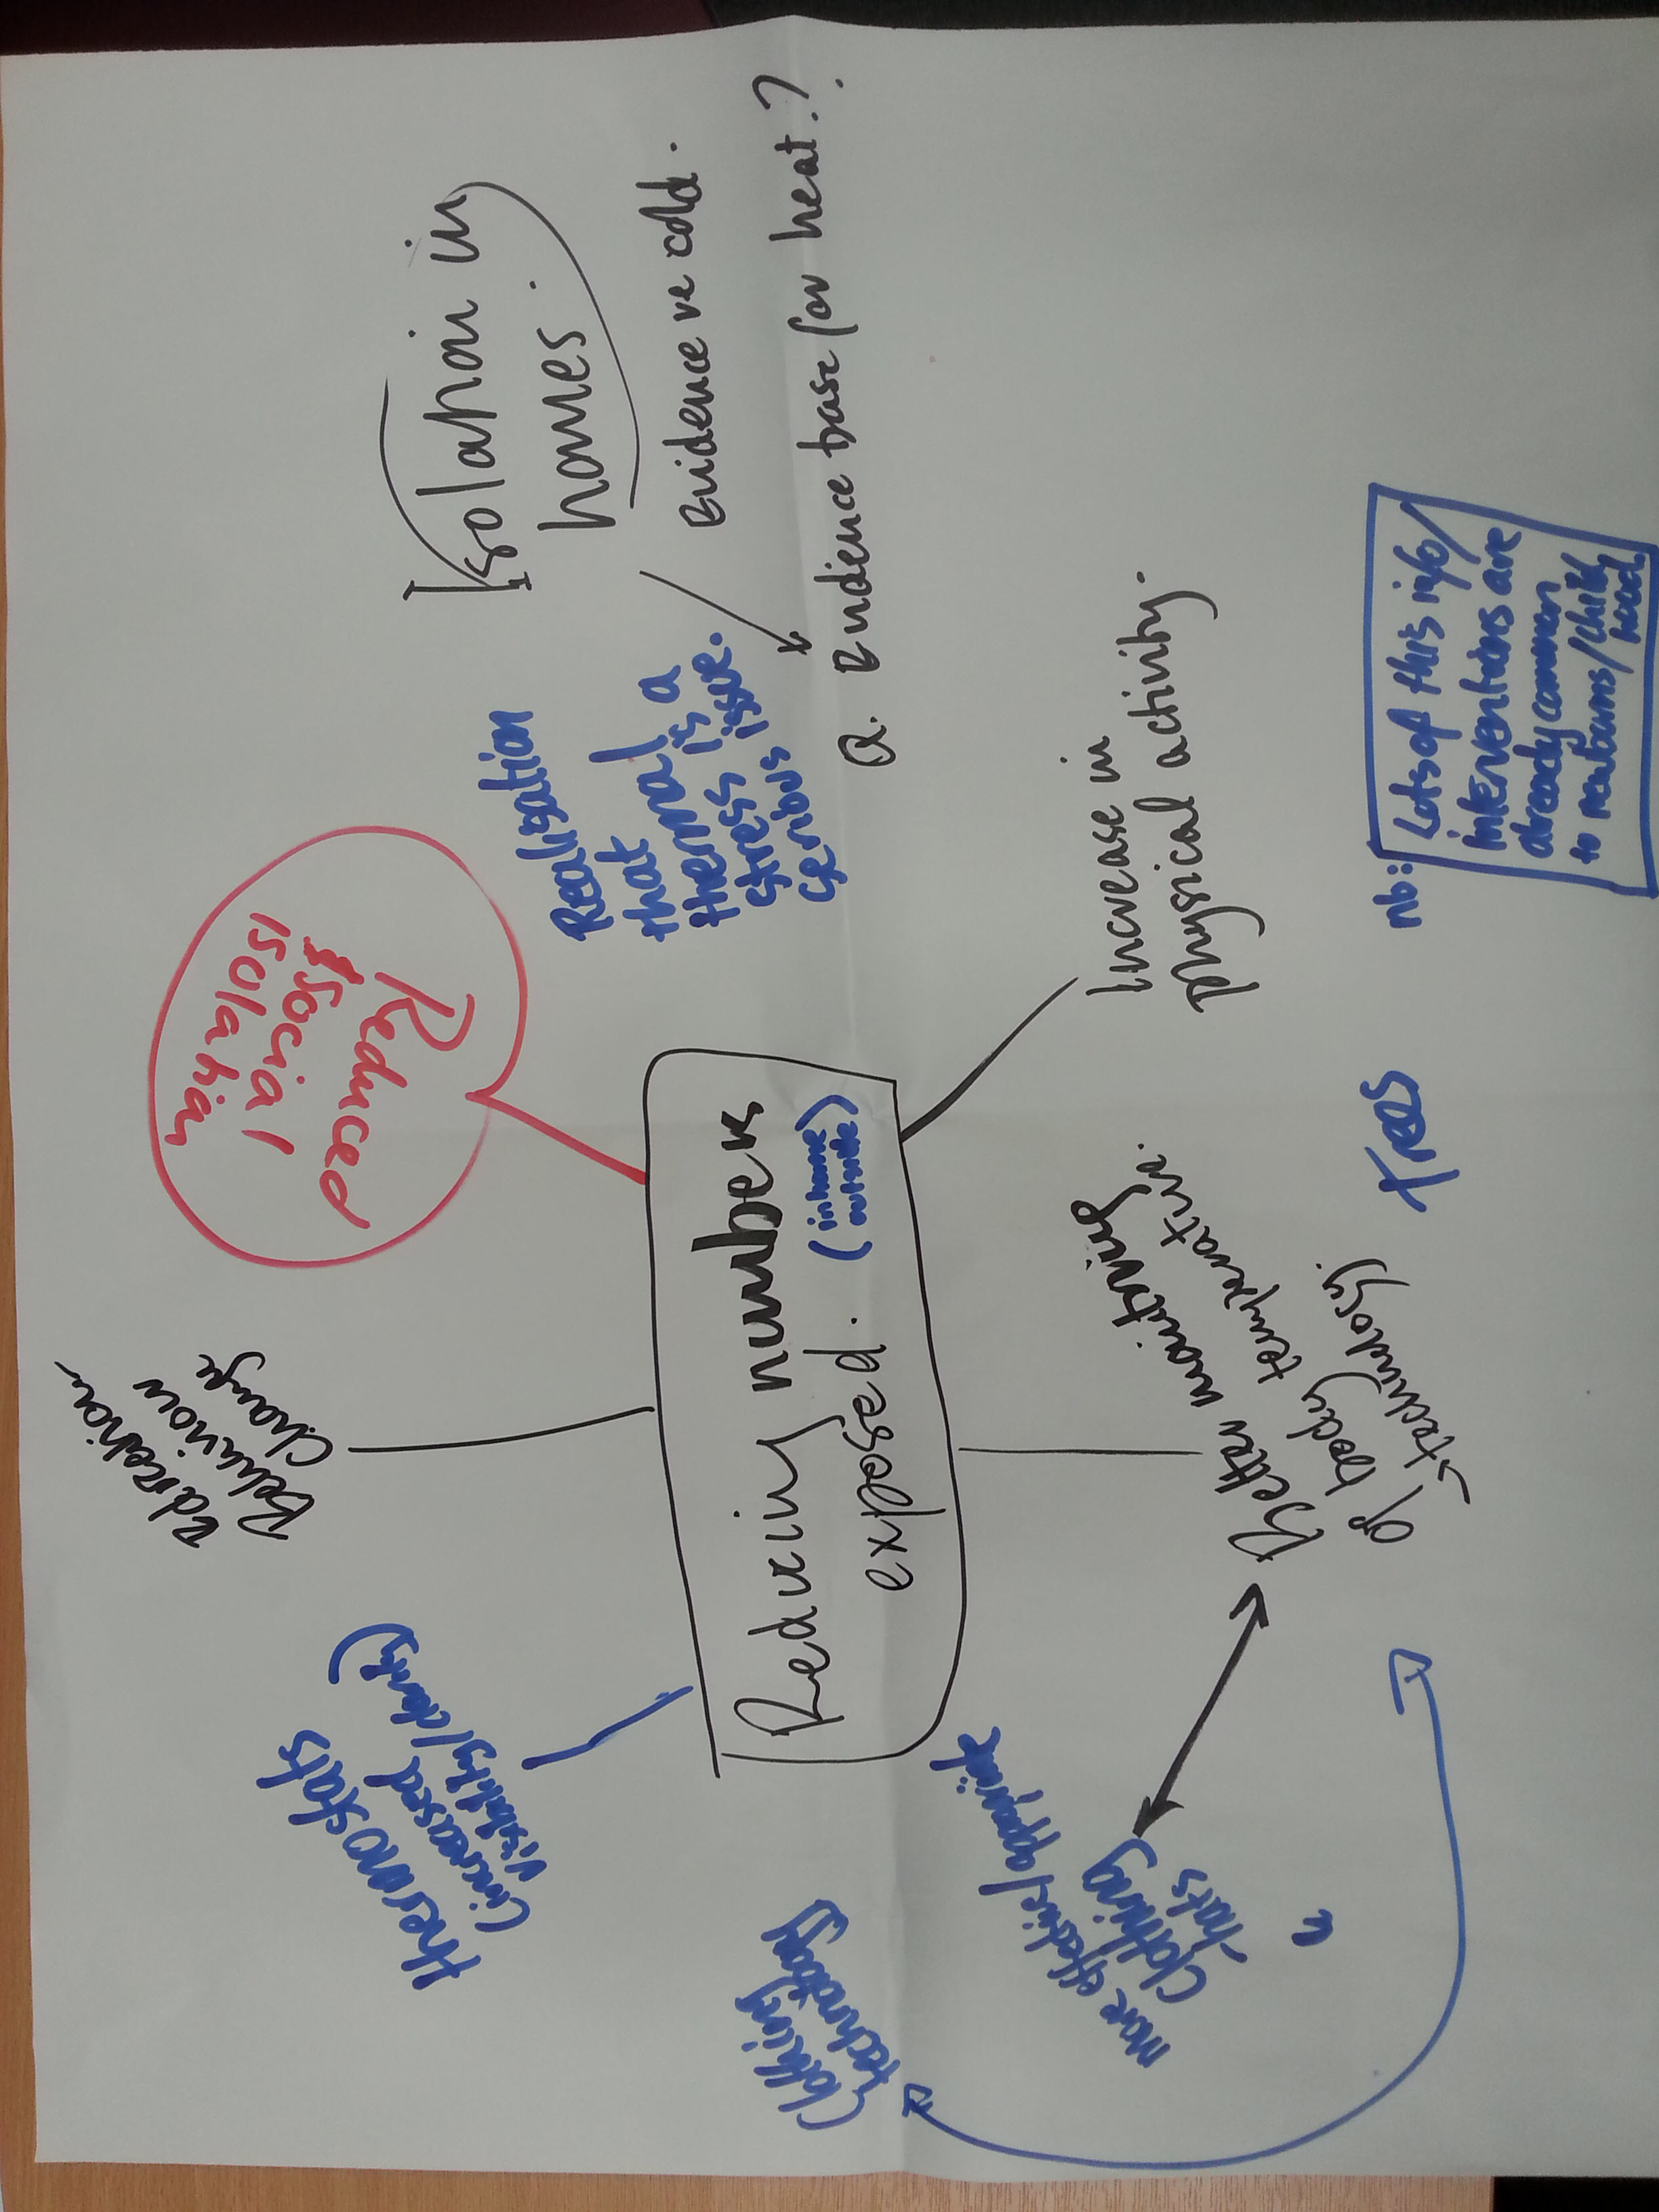
\includegraphics{img/wb7.jpg}
  \caption[Public Health Interventions: 3]{Public Health Interventions: Group 3.\label{fig:mindmap7}}
\end{figure*}

\clearpage
%this is here because LaTeX reached its limit of floats to be processed, could also put something in the preamble with new versions of LaTeX apparently.

\begin{figure*}[htpb]
 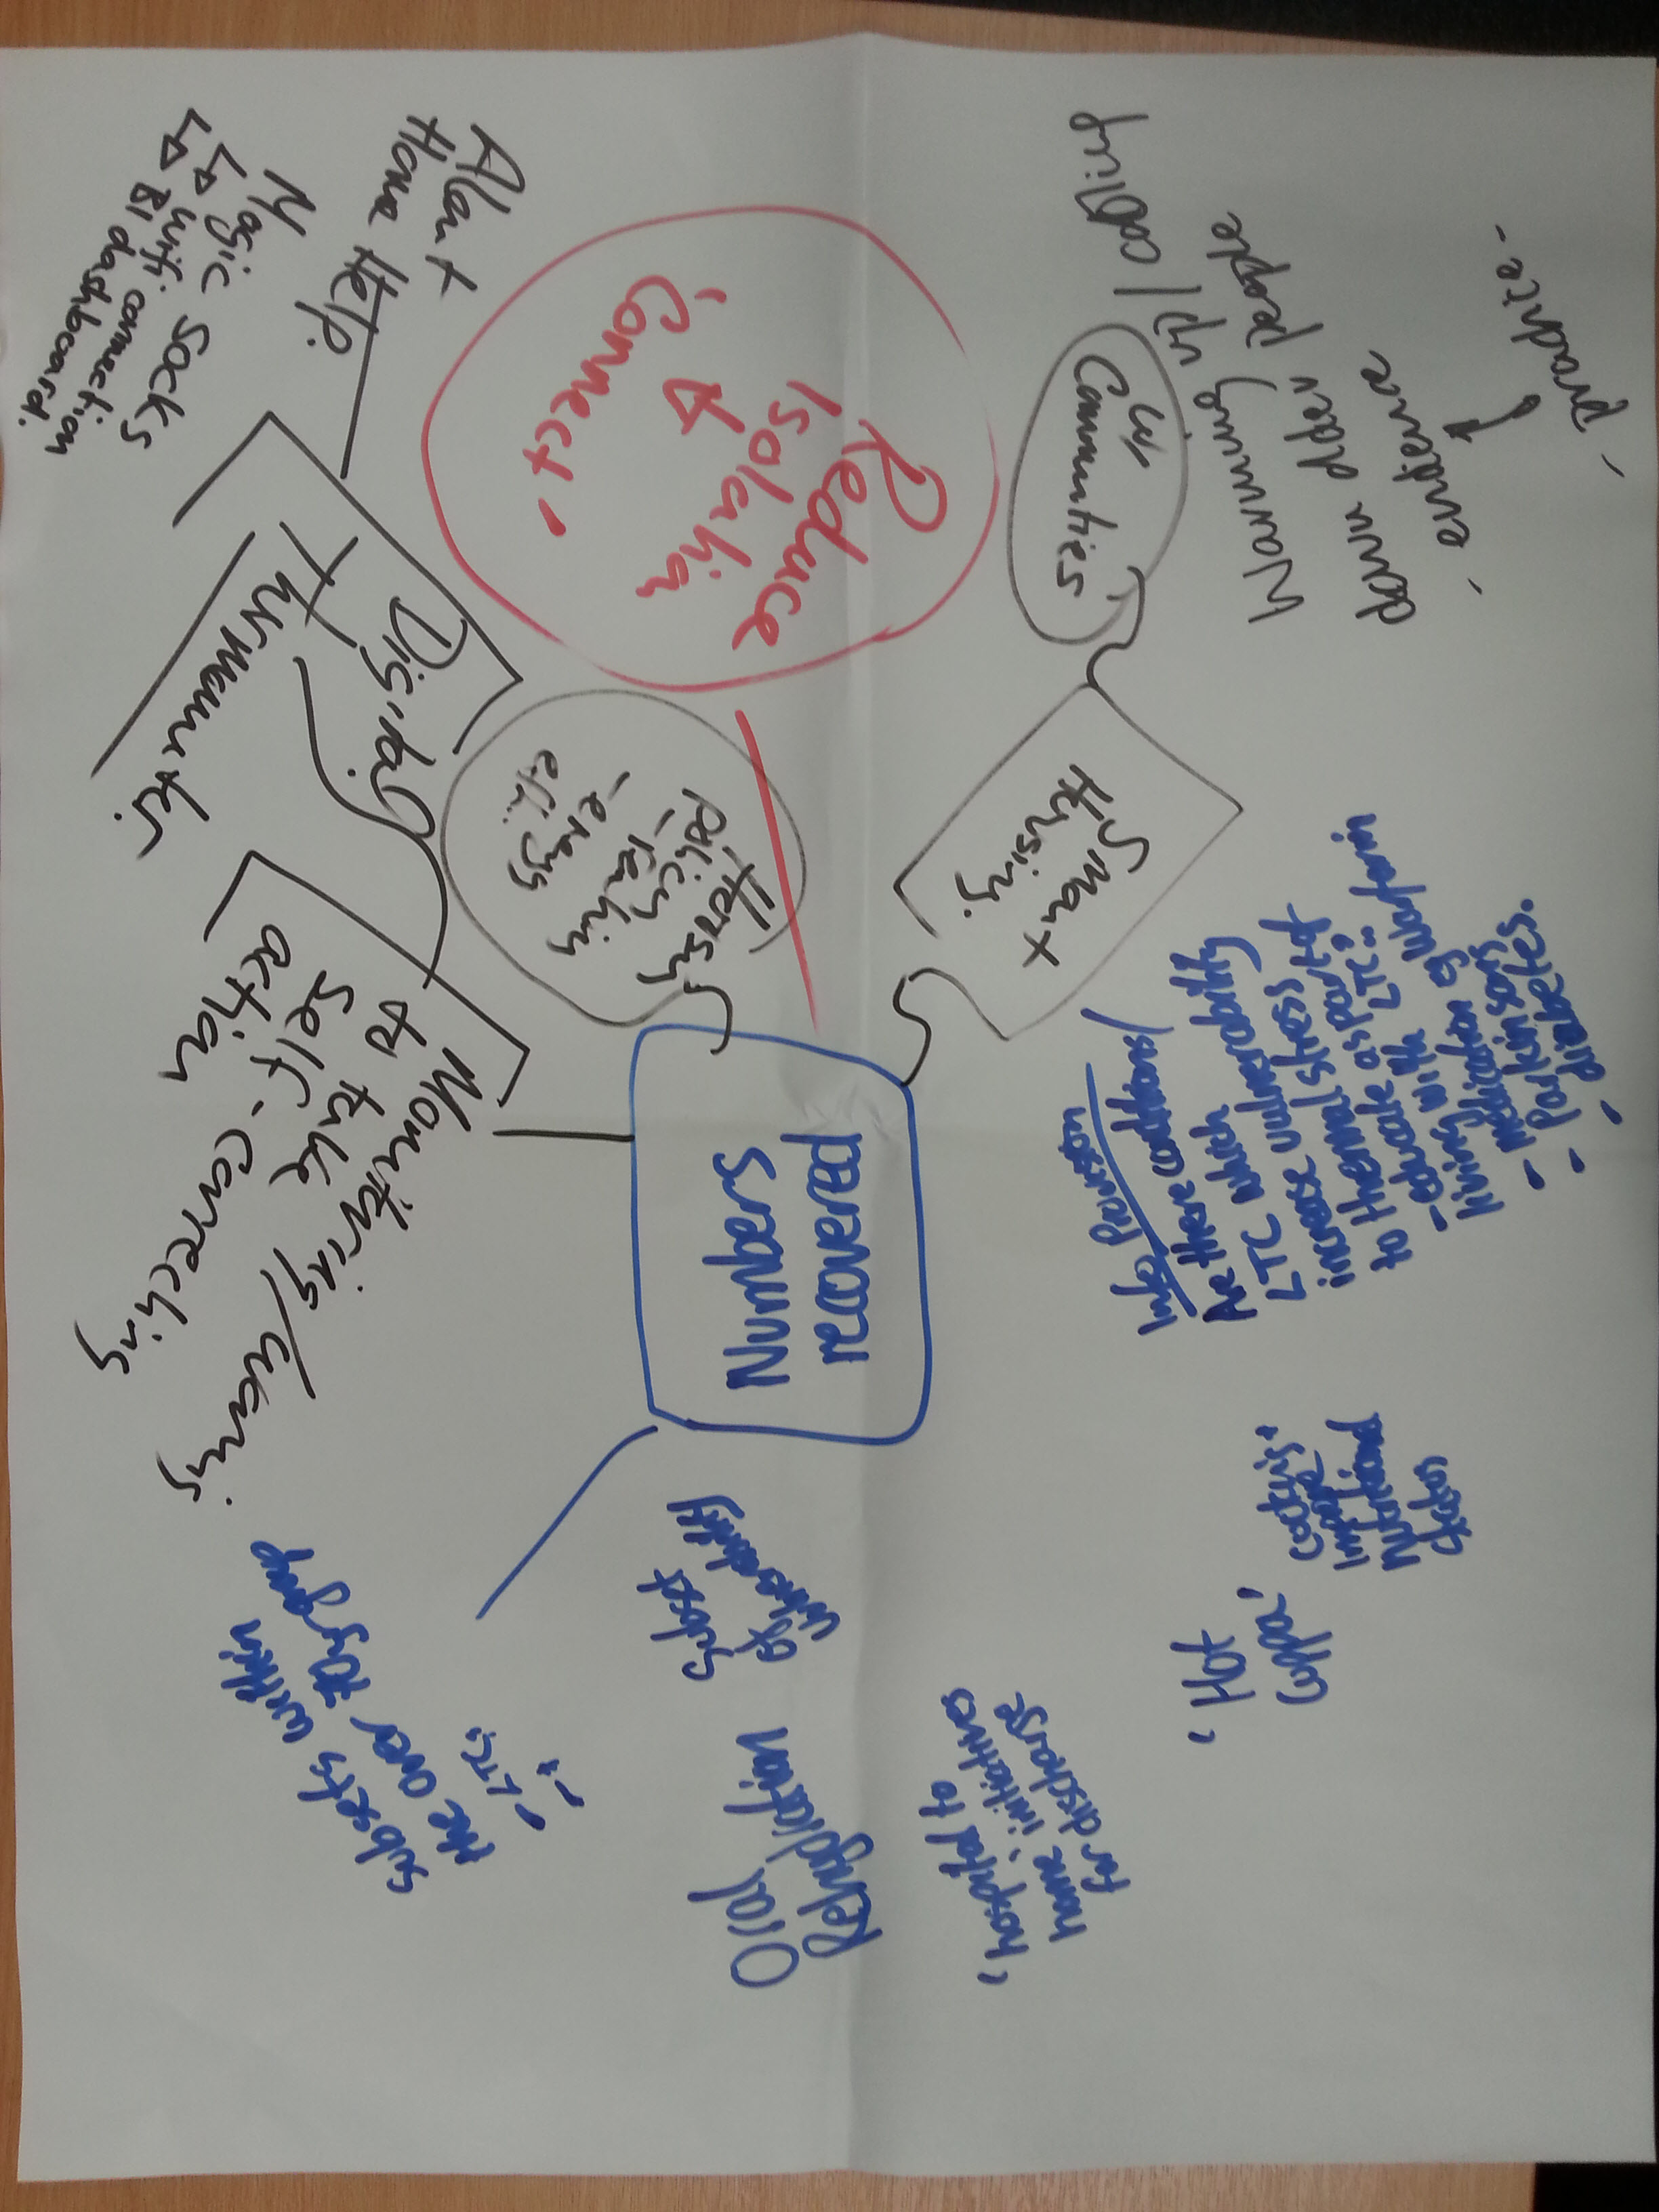
\includegraphics{img/wb8.jpg}
  \caption[Public Health Interventions: 4]{Public Health Interventions: Group 4.\label{fig:mindmap8}}
\end{figure*}


\begin{figure}[htbp]
\centering
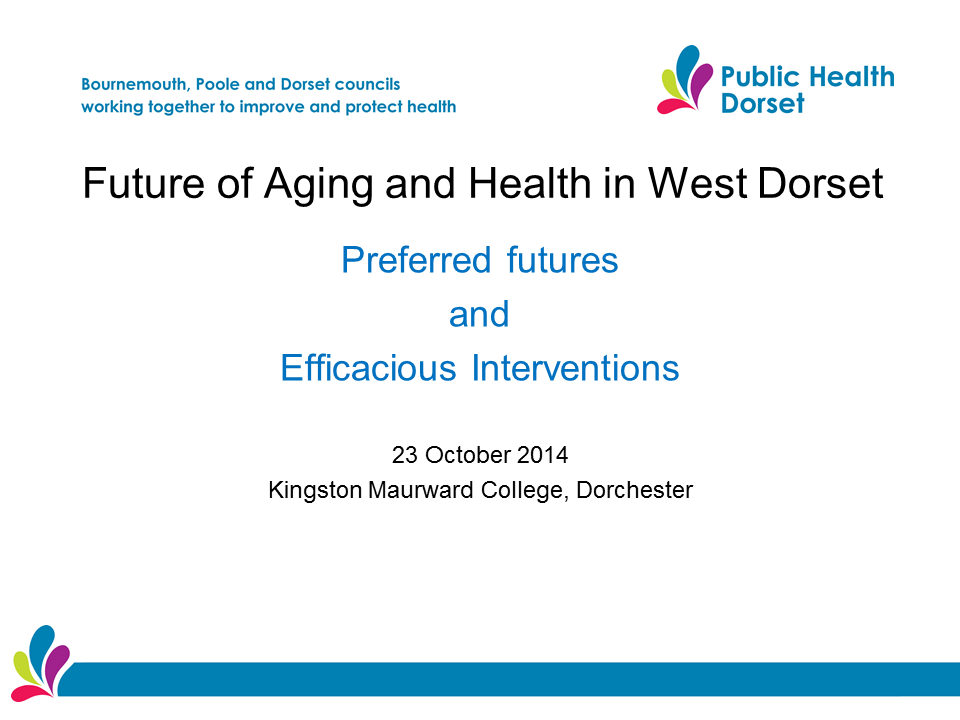
\includegraphics{img/Slide1.png}
\caption[Second Workshop Introduction]{This was the presentation to introduce and set the scene for this second workshop focussing this time on `futures studies' methods. We examine key or priority trends into the period of interest and what public health interventions might work in this context.}
\end{figure}

\begin{figure}[htbp]
\centering
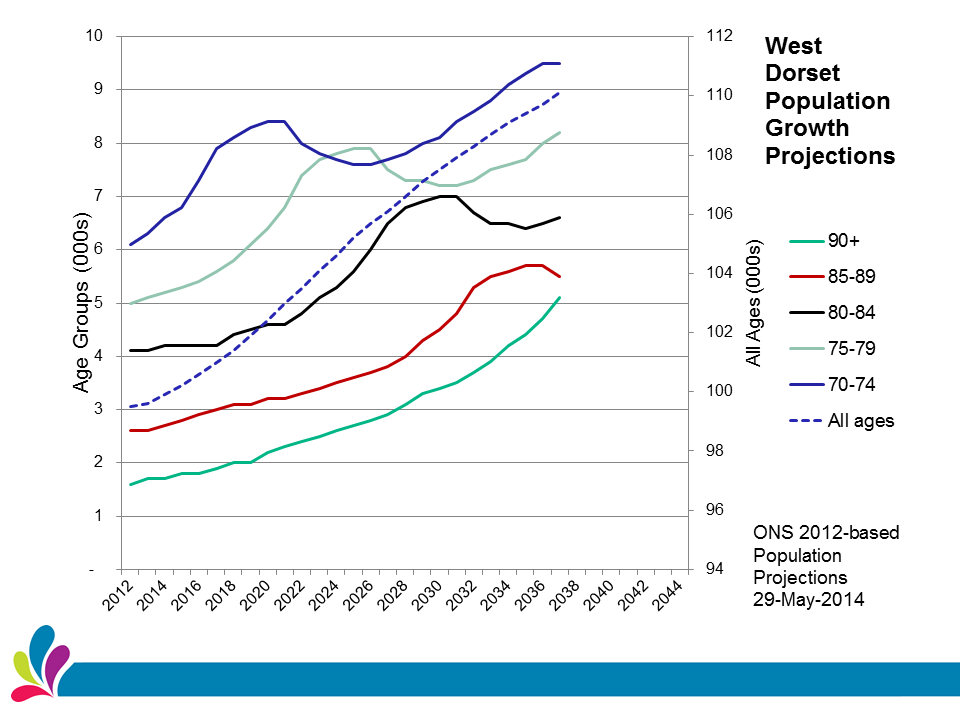
\includegraphics{img/Slide2.png}
\caption[West Dorset Population Trends]{One of the most powerful tends over the next 30 years in West Dorset will be the ageing of the population. All age population growth will be of a similar rate to that for older groups.}
\end{figure}

\begin{figure}[htbp]
\centering
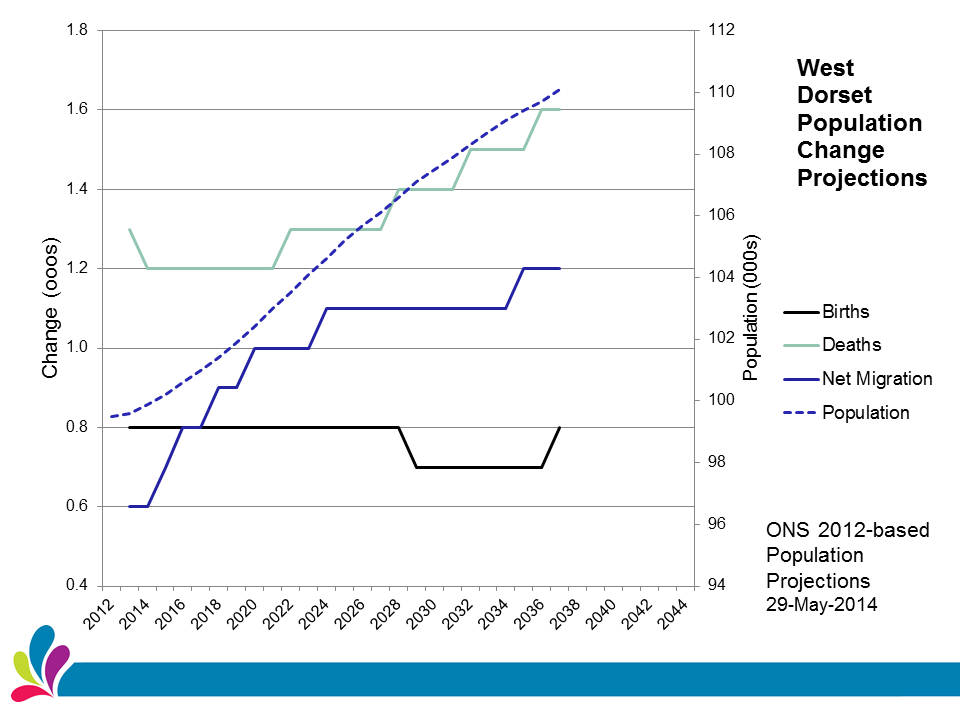
\includegraphics{img/Slide3.png}
\caption[The Role of Migration]{While births are not expected to increase in West Dorset over the next 30 years, net migration into the area will increase for the foreseeable future.}
\end{figure}


\begin{figure}[htbp]
\centering
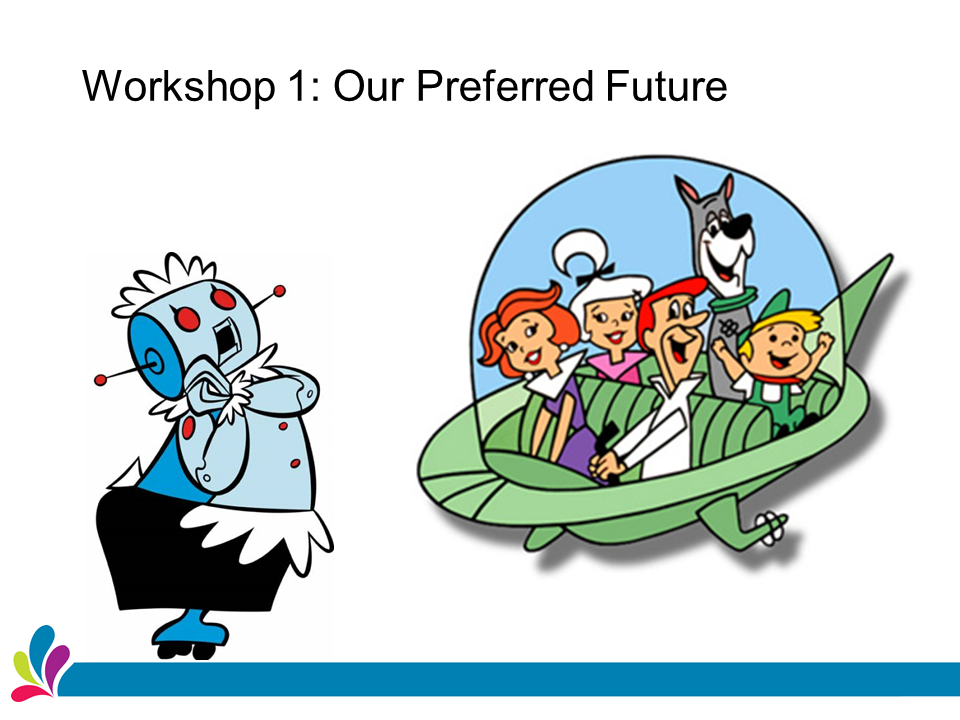
\includegraphics{img/Slide4.png}
\caption[Preferred Future Workshop Breakout 1]{Breakout groups to map out what our preferred future might be in the context of climate change in West Dorst. The essence of `future studies' is that there are many possible futures and that by understanding trends and actively moving towards a `future' that is desirable we start living strategies and not just writing them down and hoping for the best.}
\end{figure}

\begin{figure}[htbp]
\centering
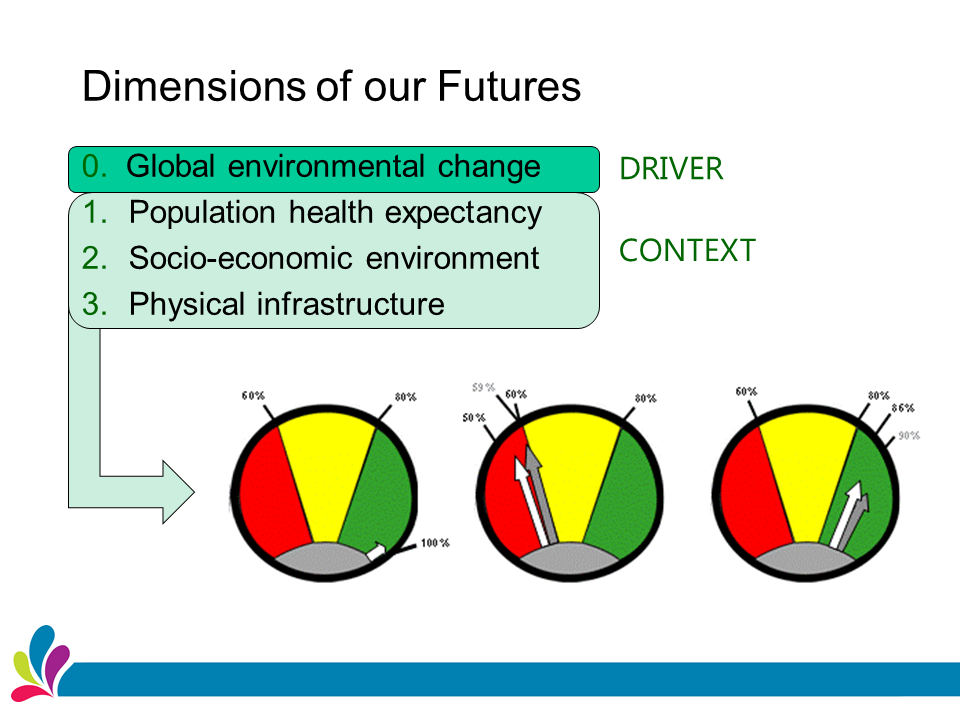
\includegraphics{img/Slide5.png}
\caption[Putting drivers/trends to work]{Identification of key drivers/trends can be used to `indicate' future states of things we don't necessarily see trends in, allowing us to build up a systems picture of possible futures.}
\end{figure}

\begin{figure}[htbp]
\centering
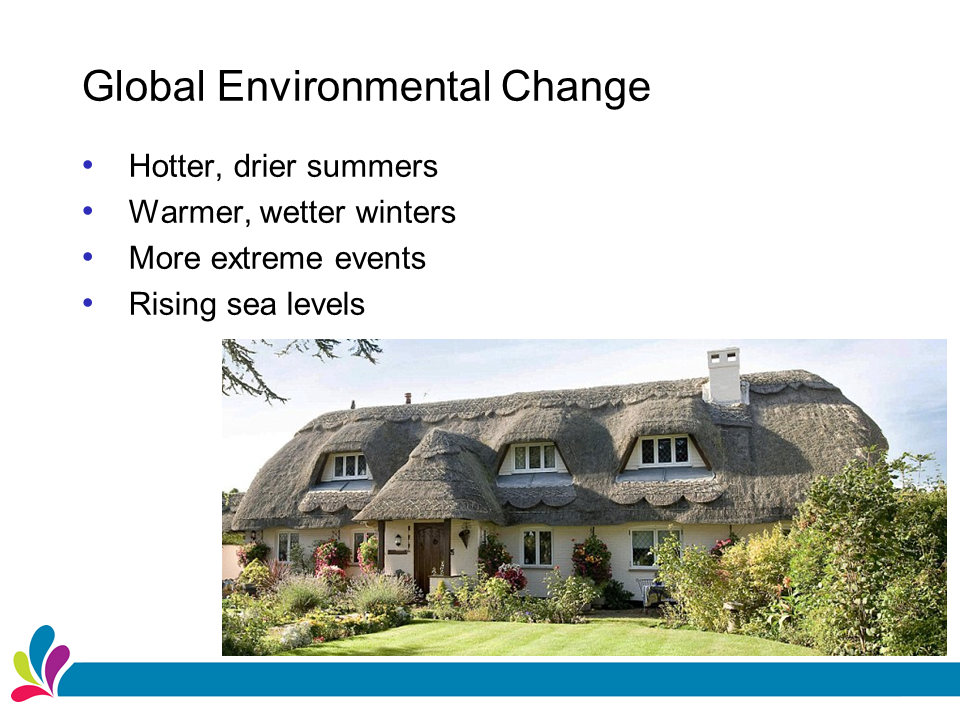
\includegraphics{img/Slide6.png}
\caption[Global Environmental Change]{Even if we have a great deal of confidence in key global environmental trends, it's the context that we need to be aware of for local communities. And it seems completely obvious that this depends on which end of the socio-economic spectrum you sit.}
\end{figure}

\begin{figure}[htbp]
\centering
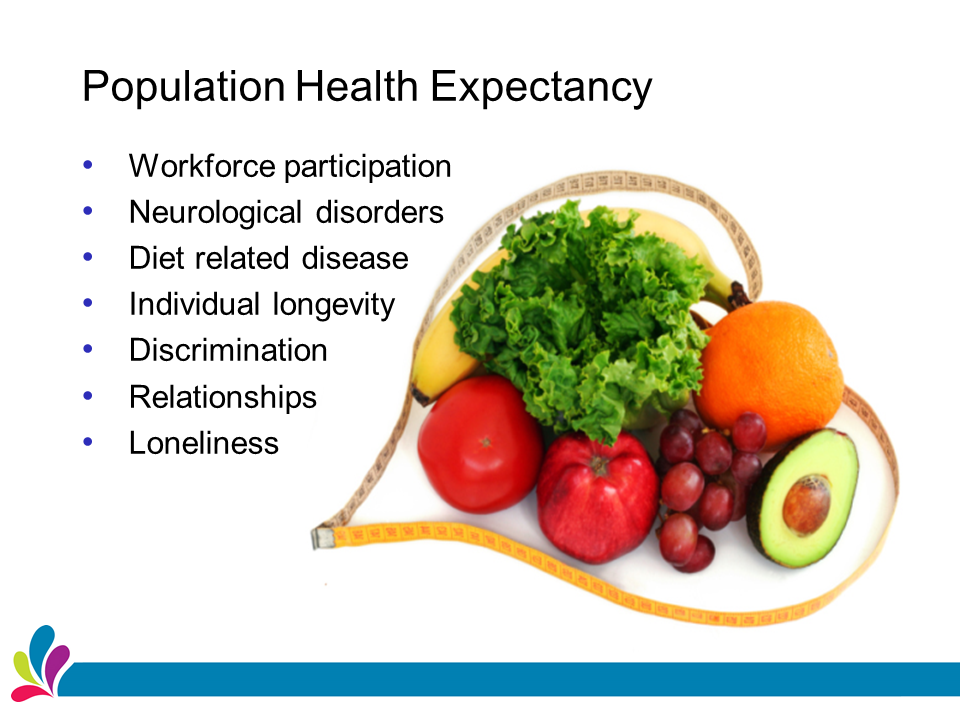
\includegraphics{img/Slide7.png}
\caption[Population Health Expectancy]{Even when we are focusing on a health impact as `simple' as thermal stress, there are a number of co-factors/confounders that play a role in determining how large an impact there will be.}
\end{figure}

\begin{figure}[htbp]
\centering
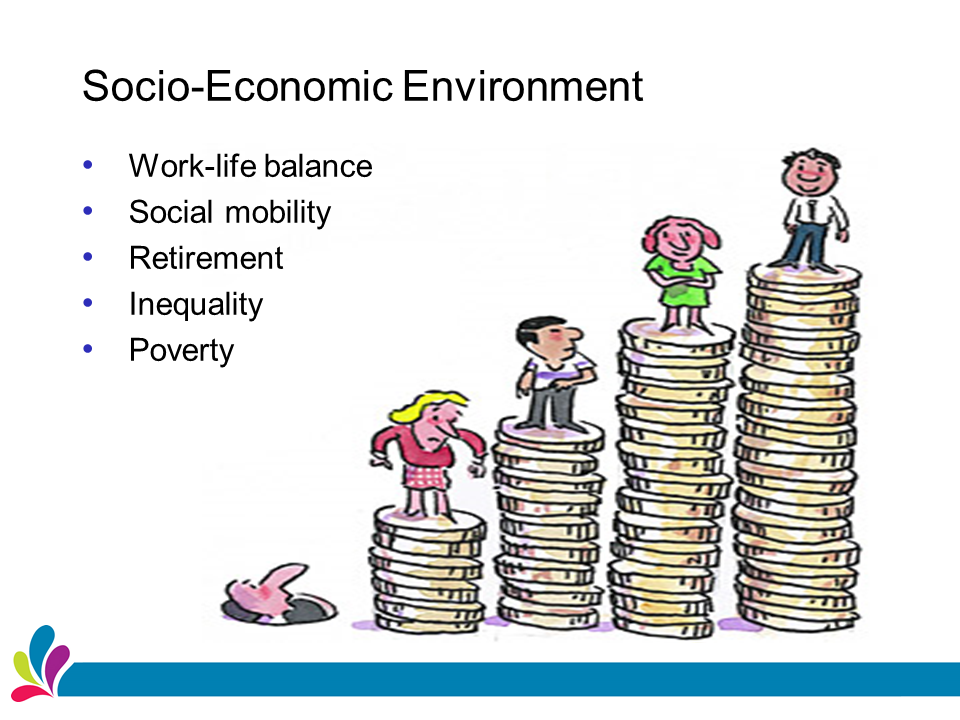
\includegraphics{img/Slide8.png}
\caption[Socio-Economic Environment]{Aspects of who we are, what the population looks like, are dependent on non-physical and non-health factors, factors that can mitigate impact and increase resilience.}
\end{figure}

\begin{figure}[htbp]
\centering
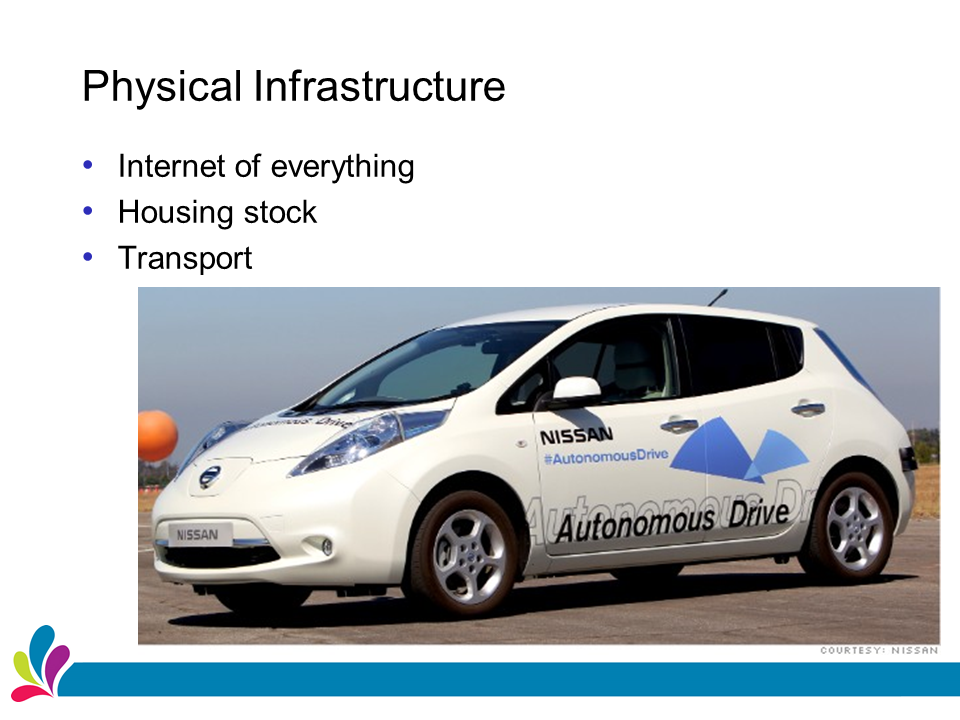
\includegraphics{img/Slide9.png}
\caption[Physical Infrastructure]{Physical infrastructure is an important consideration in futures we might imagine, especially where information is more easily obtained and used to prevent health impacts.}
\end{figure}

\begin{figure}[htbp]
\centering
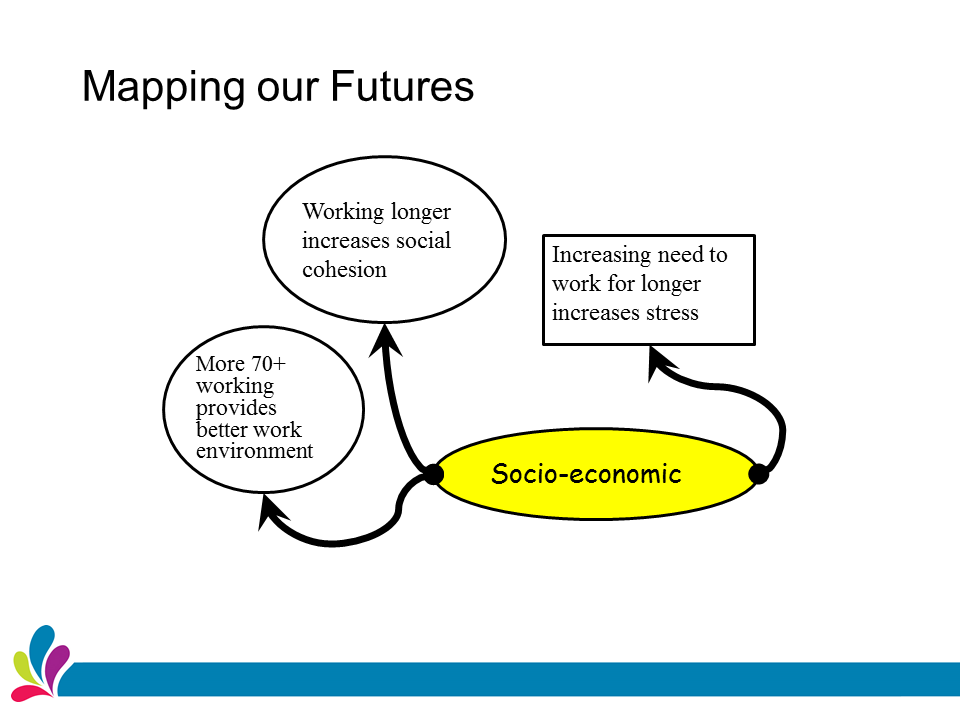
\includegraphics{img/Slide10.png}
\caption[Mapping our Futures]{Mapping our possible futures allows us to visually set our causal pathways to both impact and resilience. ``If this, then that'' is a useful construct in imagining how we might structure our future to improve wellbeing.}
\end{figure}

\begin{figure}[htbp]
\centering
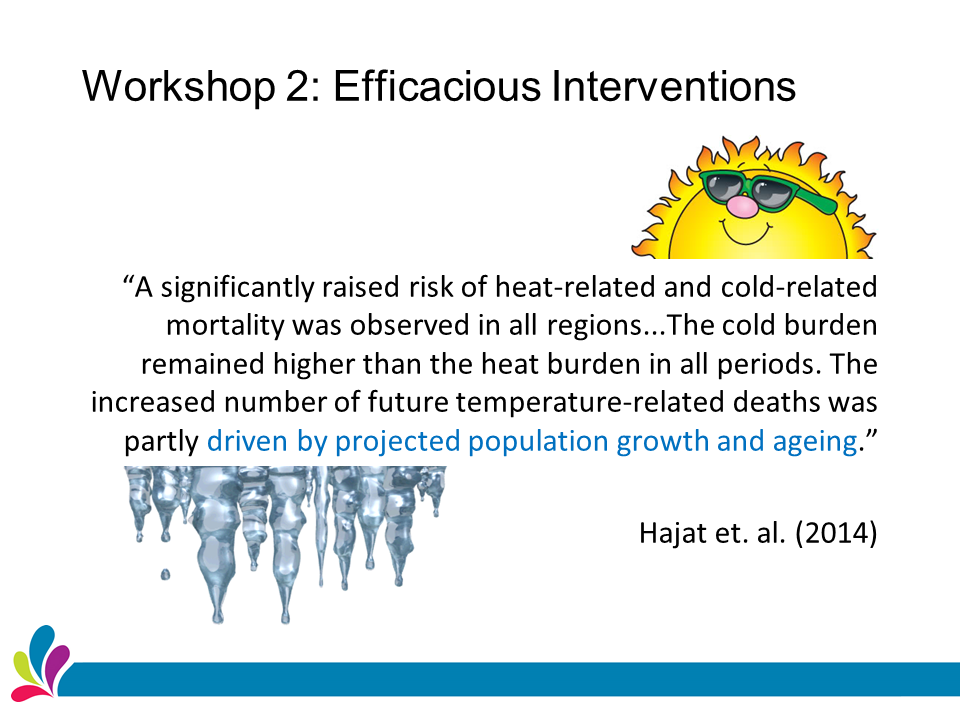
\includegraphics{img/Slide11.png}
\caption[Efficacious Interventions Workshop Breakout 2]{A second workshop session of small groups was held to brain storm public health interventions in the context of what we imagine the future might look like.}
\end{figure}

\begin{figure}[htbp]
\centering
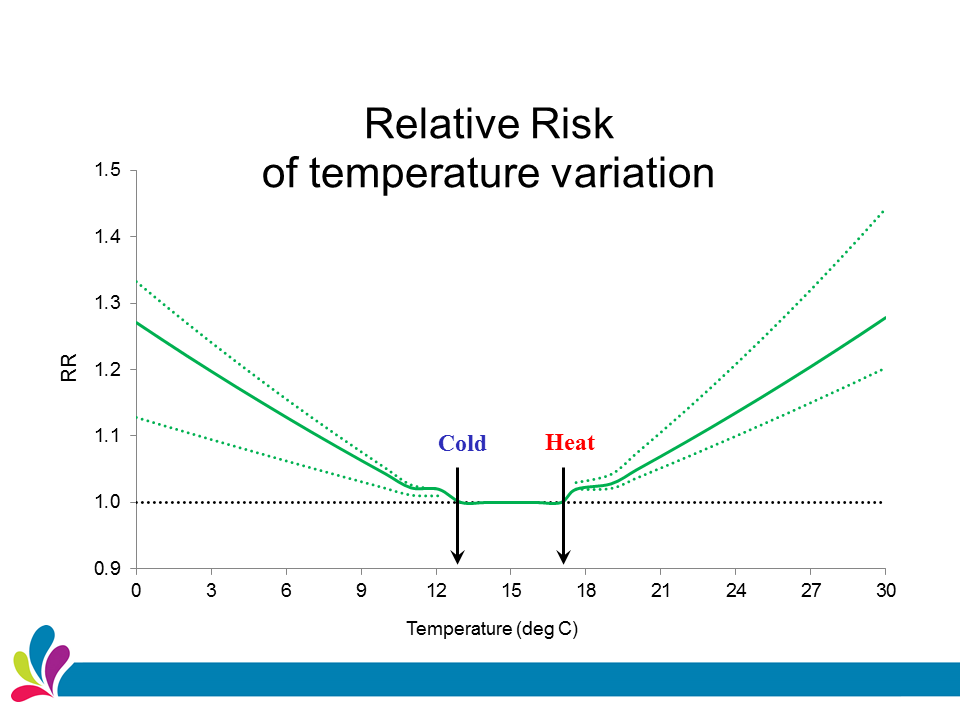
\includegraphics{img/Slide12.png}
\caption[Relative Risk in Thermal Stress]{At the core of our modelling is a very simple relationship between thermal stress and relative risk of dying. For the West Dorset population, if you exceed 17.6\textdegree C or drop below 12.1\textdegree C you are thermally stressed. A statistical relationship between age specific mortality and temperature identifies these thresholds and the linear relationships outside of them, with confidence intervals.}
\end{figure}

\begin{figure}[htbp]
\centering
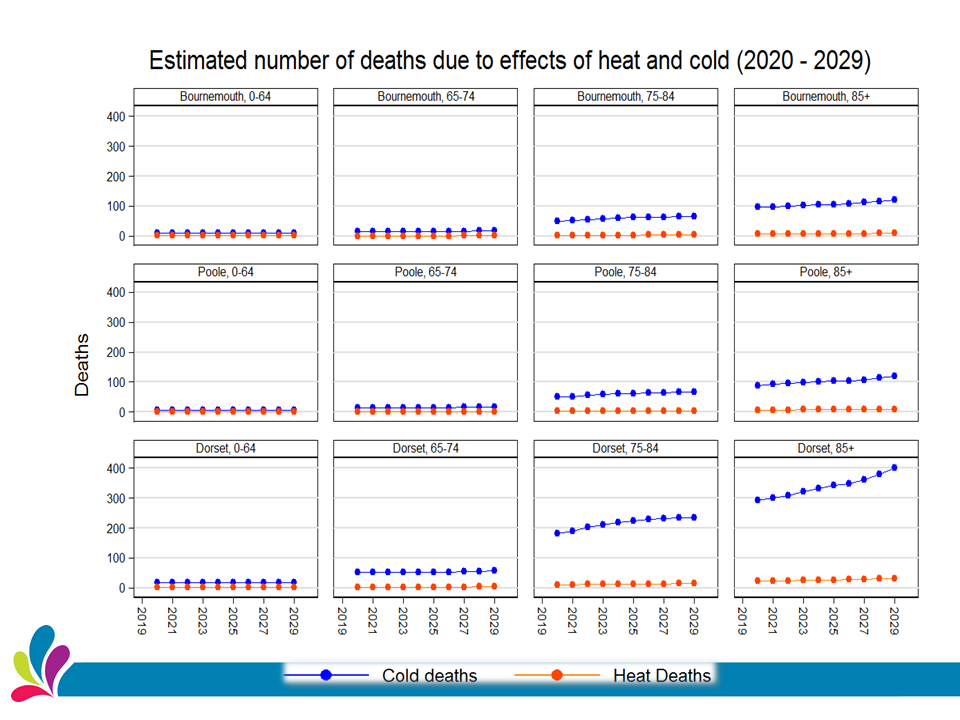
\includegraphics{img/Slide13.png}
\caption[Deaths Due to Thermal Stress, 2020-2029]{Looking at the estimated temperatures of a `warmer world' in the period 2020-2029 (for which we have climate model simulations) we can estimate `excess mortality' by age group for both cold and heat stress. It comes as a bit of a surprise to people that cold stress related mortality increases will be greater than heat stress related mortality. The power of the population ageing trend.}
\end{figure}

\begin{figure}[htbp]
\centering
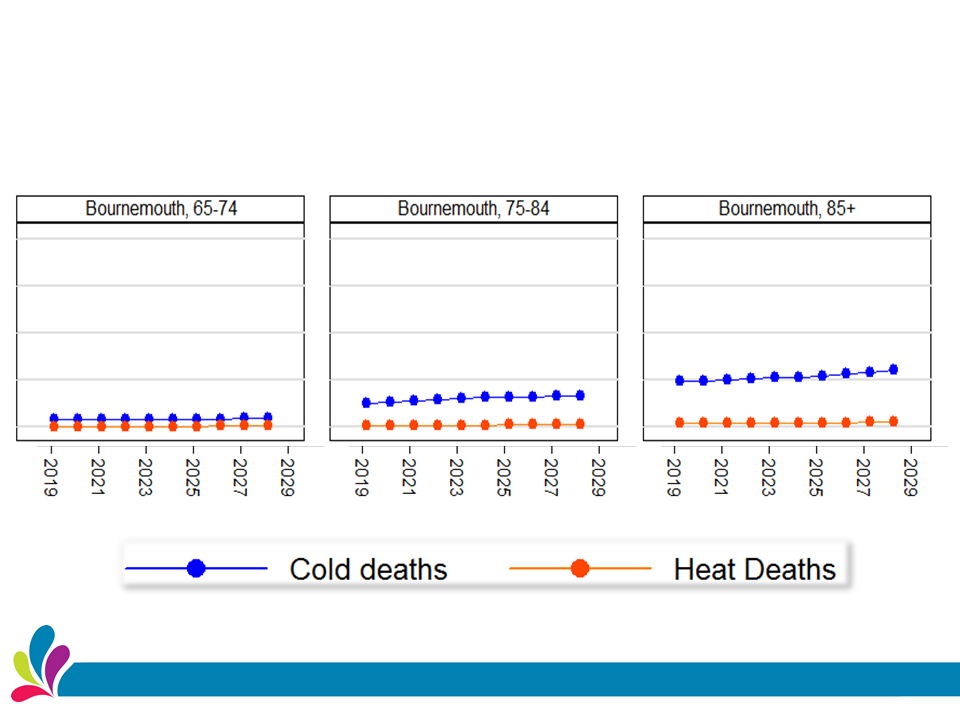
\includegraphics{img/Slide14.png}
\caption[Bournemouth Deaths, 2020-2029]{Bournemouth thermal stress related deaths, 2020-2029}
\end{figure}

\begin{figure}[htbp]
\centering
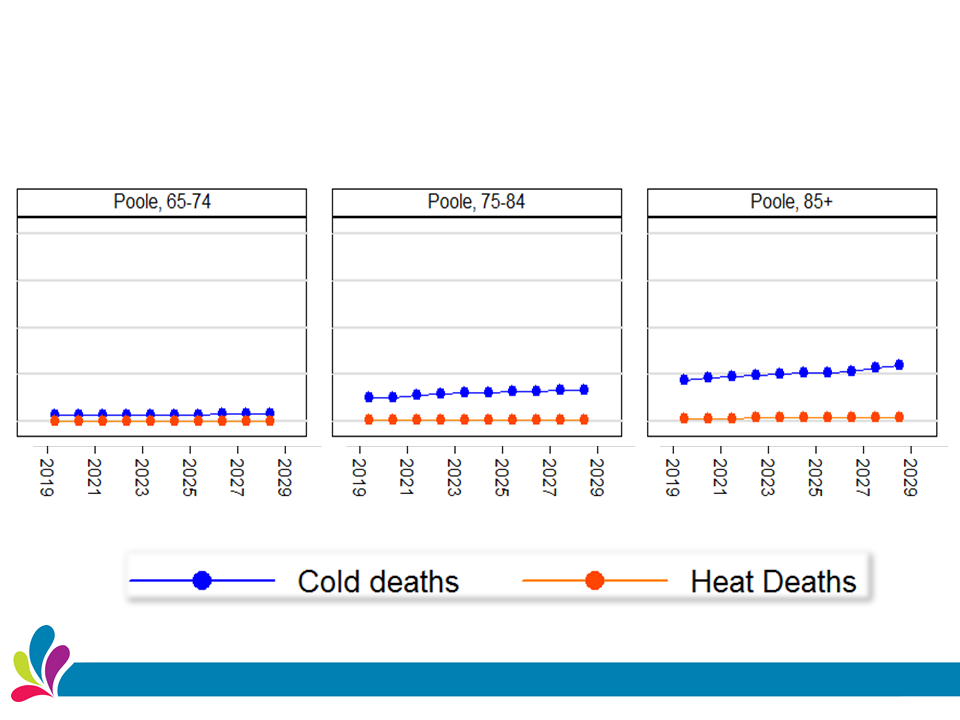
\includegraphics{img/Slide15.png}
\caption[Poole Deaths, 2020-2029]{Poole thermal stress related deaths, 2020-2029}
\end{figure}

\begin{figure}[htbp]
\centering
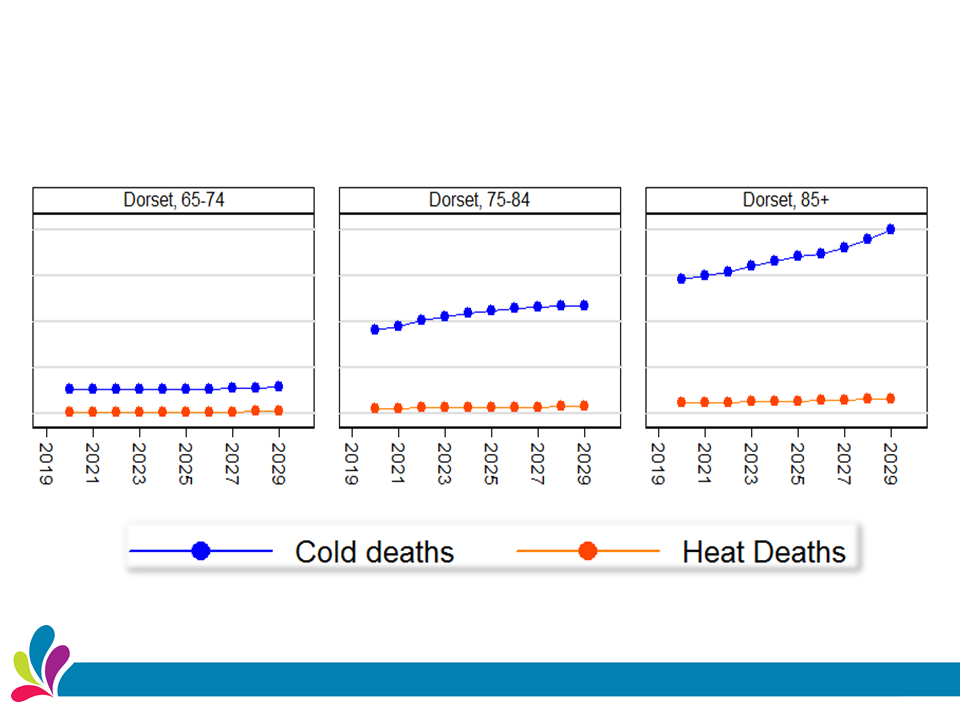
\includegraphics{img/Slide16.png}
\caption[Dorset Deaths, 2020-2029]{Dorset thermal stress related deaths, 2020-2029}
\end{figure}

%\clearpage
%this is here because LaTeX reached its limit of floats to be processed, could also put something in the preamble with new versions of LaTeX apparently.

\begin{figure}[htbp]
\centering
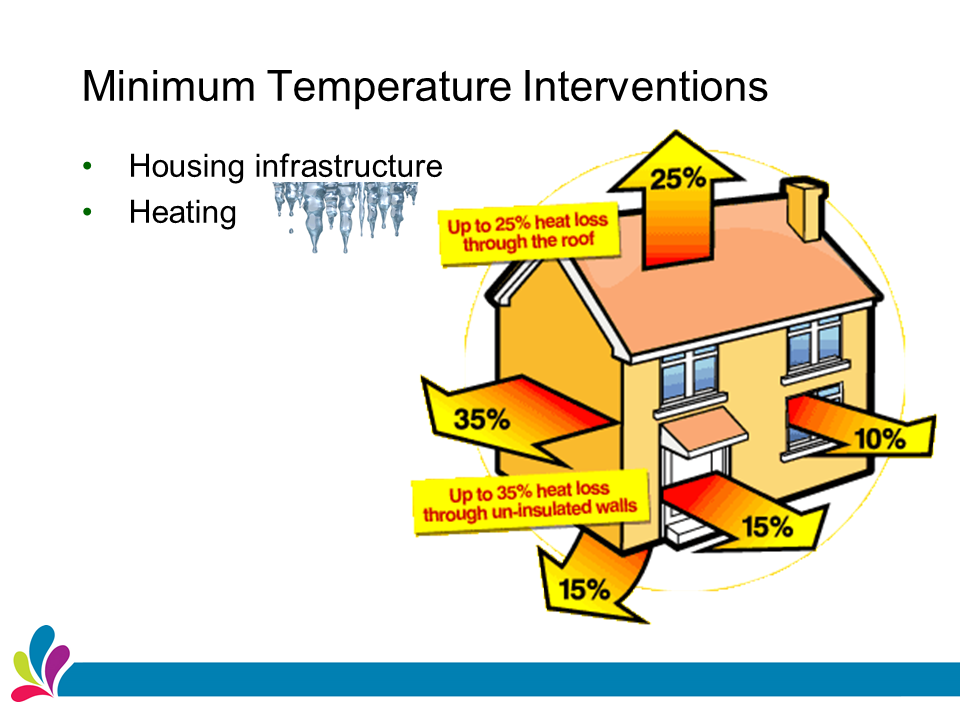
\includegraphics{img/Slide17.png}
\caption[Minimum Temperature Interventions]{Minimum Temperature Interventions might include future housing `eco' designs and also more efficient heating systems.}
\end{figure}

\begin{figure}[htbp]
\centering
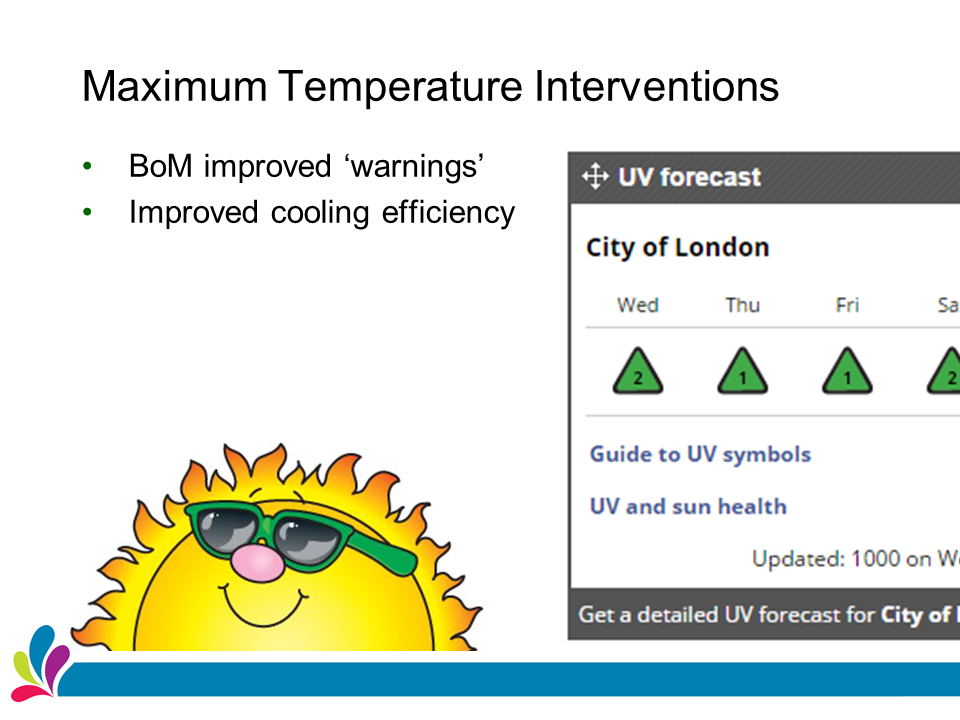
\includegraphics{img/Slide18.png}
\caption[Maximum Temperature Interventions]{Maximum Temperature Interventions might include improved heat wave warnings and improved cooling design of housing, workplaces, clothing, etc.}
\end{figure}


\begin{figure}[htbp]
\centering
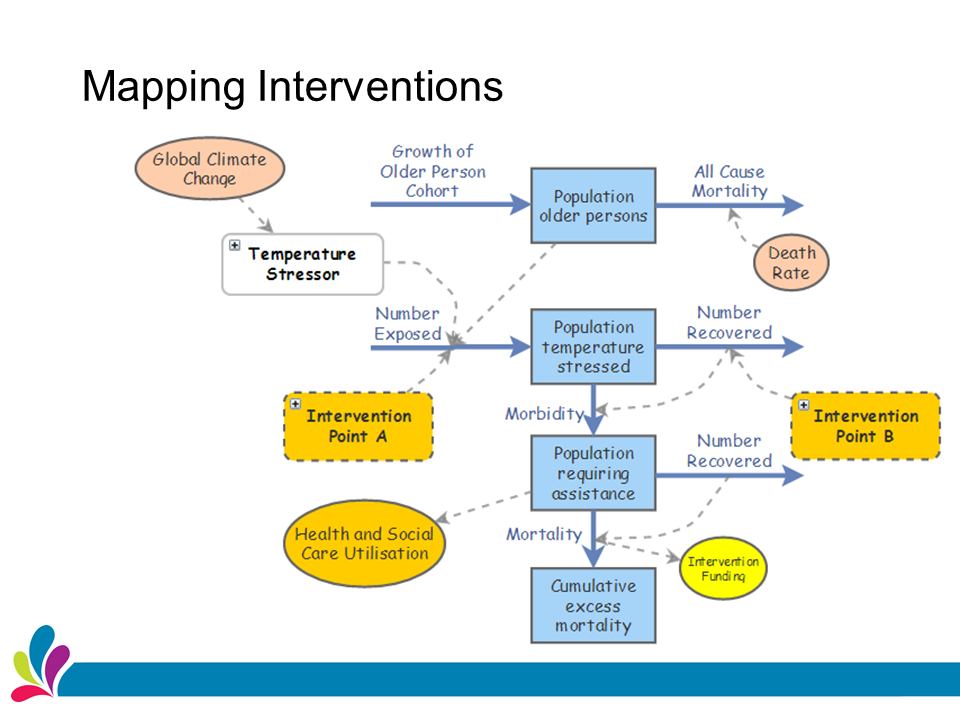
\includegraphics{img/Slide19.png}
\caption[Mapping Interventions]{The power of systems maps and systems thinking comes in the ability to visualise and eventually `game' different interventions.}
\end{figure}



